\chapter{Software Evolution in Real-world}
\label{chap:evolution}

The multi-version execution approach is based on two key assumptions.  First,
that new bugs are being introduced during software evolution and maintenance
process even to a well tested code. Second, that during software evolution,
the externally observable behaviour of the applications remains relatively
stable, especially between minor revisions (\ie security and bug fixes).  While
there is a lot of first hand and anecdotal evidence in support of these
assumptions, despite the key role that software evolution plays in the
application life cycle, it is surprising how few empirical studies one can find
in the research literature regarding the co-evolution of test suites and code
and their impact on the \emph{execution} of real systems.

Software repositories provide rich information about the construction and
evolution of software systems. While static data extracted from software
repositories have been extensively studied, dynamic metrics concerning the
execution of the software have received much less attention, due to the
inherent difficulty of running and monitoring a large number of software
versions.

In this chapter, we present an empirical study concerning dynamic metrics which
aims to answer some of the questions related to software evolution. To perform
this study, we have built a flexible infrastructure that can be used to run
each version of a system in isolation and collect static and dynamic software
metrics, using a lightweight virtualization environment based on software
containers, that can be deployed on a cluster of local or cloud machines.

We have used this infrastructure to examine how code and tests co-evolve in
\numSystems popular open-source systems. We report the main characteristics of
software patches, analyse the evolution of program and patch coverage, assess
the impact of non-determinism on the execution of test suites, and investigate
whether the coverage of code containing bugs and bug fixes is higher than
average.

% While static metrics can provide useful insights into the construction and
% evolution of software, there are many software engineering aspects which
% require information about software executions.  For example, the research
% community has invested a lot of effort in designing techniques for improving
% the testing of software patches, ranging from test suite prioritisation and
% selection
% algorithms~\cite{harrold:test-redundancy,test-pri,Rothermel96analyzingregression}
% to program analysis techniques for test case generation and bug
% finding~\cite{diff-symex,directed-test-augmen:09,express,directed-symex11,babic11,directed-incr-symex11,patch:spin12,interaction-changes13}.

% Many of these techniques depend on the existence of a manual test suite,
% sometimes requiring the availability of a test exercising the
% patch~\cite{onlinevalidation,tachyon12}, sometimes making assumptions about the
% stability of program coverage or external behaviour over
% time~\cite{cov_regr97,mx}, other times using it as a starting point for
% exploration~\cite{zesti,pretex,sage,test-augmentation:genetic-vs-concolic}, and
% often times employing it as a baseline for
% comparison~\cite{klee,dotnet-random-test08,semantic-fp-testing12,mutation-tests-oracle12}.
% However, despite the key role that test suites play in software testing, it is
% surprising how few empirical studies one can find in the research literature
% regarding the co-evolution of test suites and code and their impact on the
% \emph{execution} of real systems.

% In this chapter, we present \covrig, a flexible infrastructure that can be used
% to run each version of a system in isolation and collect static and dynamic
% software metrics, using a lightweight virtual machine environment that can be
% deployed on a cluster of local or cloud machines.

% We use \covrig to conduct an empirical study examining how code and tests
% co-evolve in \numSystems popular open-source systems.  We report the main
% characteristics of software patches, analyse the evolution of program and patch
% coverage, assess the impact of non-determinism on the execution of test suites,
% and investigate whether the coverage of code containing bugs and bug fixes is
% higher than average.

% We use \covrig to conduct an empirical study examining how programs evolve in
% terms of code, tests and coverage.  More precisely, we have analysed the
% evolution of \numSystems popular software systems with a rich development
% history over a combined period of \numYears years, with the goal of answering
% the following list of research questions (RQs):

% \begin{itemize}
% \item[\textssc{RQ1}] \textit{\rqone}
%             Are coding and testing continuous, closely linked
%             activities?  Or do periods of intense development
%             alternate with periods of testing?

% \item[\textssc{RQ2}] \textit{\rqtwo}
%             Are most code
%             patches accompanied by a new or modified test case?  How
%             many patches modify neither executable code nor tests?
           
% \item[\textssc{RQ3}] \textit{\rqthree}
%             Are most patches small?  
%             How many different parts of the code does a patch touch?
%             What is the median number of lines, hunks and
%             files affected by a patch?

% \item[\textssc{RQ4}] \textit{\rqfour}  Do tests fail non-deterministically?
%             Does running the test suite multiple times cover different
%             lines of code?

% \item[\textssc{RQ5}] \textit{\rqfive}
%             Does the overall coverage increase steadily over time, or
%             does it remain constant?  Are there revisions that
%             significantly increase or decrease coverage?

% \item[\textssc{RQ6}] \textit{\rqsix}
%             What fraction of a patch is covered by the regression test
%             suite?  Does patch coverage depend on the size of the
%             patch?

% \item[\textssc{RQ7}] \textit{\rqseven}  Are
%             tests exercising recent patches added shortly after the
%             patch was submitted?  If so, how significant is this
%             latent patch coverage?

% \item[\textssc{RQ8}] \textit{\rqeight}
%             Are most fixes thoroughly exercised by the regression
%             suite?  How many fixes are entirely executed?

% \item[\textssc{RQ9}] \textit{\rqnine}
%             Is code that contains bugs exercised less than other changes?
%             Is coverage a reasonable indicator of code quality? 

% %\item[\bf RQ10:] \textbf{Does buggy code have lower than average coverage?}
% \end{itemize}

\section{Study infrastructure}
\label{sec:design}

\begin{figure}[t!]
\centering
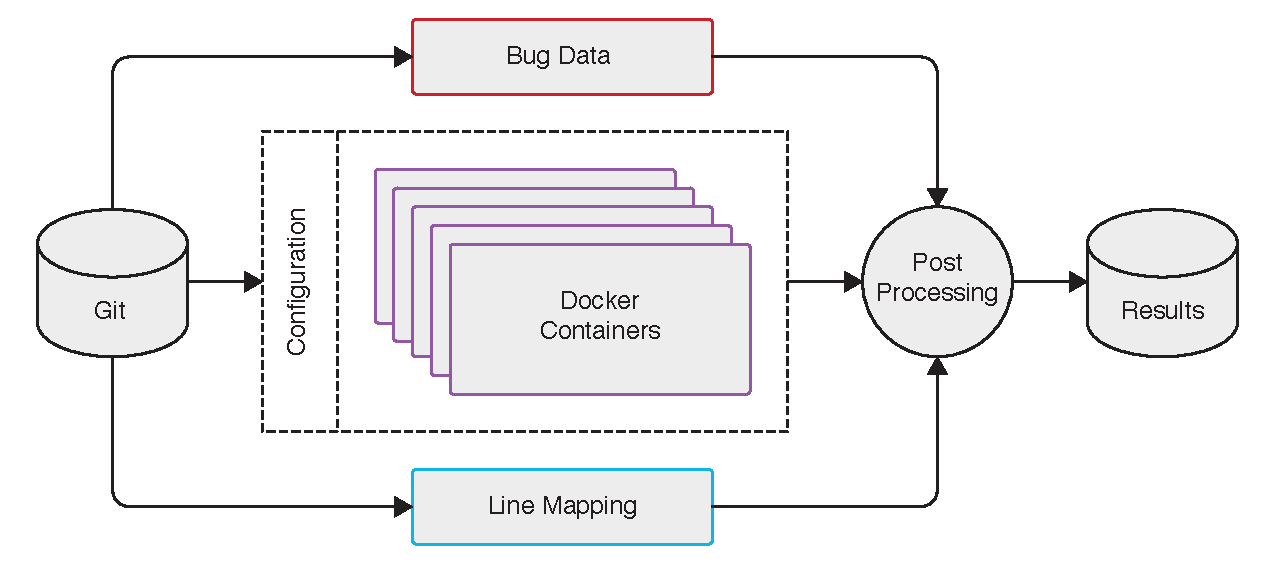
\includegraphics[width=0.75\textwidth]{evolution/figures/pipeline}
\caption{The architecture of the infrastructure used in the empirical study.}
\label{fig:arch}
\end{figure}

The overall architecture of the infrastructure used in our study is depicted in
Figure~\ref{fig:arch}.  It contains a generic driver which iterates through all
the revisions in a given range and invokes routines specific to each system to
compile, run, and collect statistics of interest.

%% To collect information about each program revision, such as whether it
%% successfully compiles, whether it passes the regression tests and with
%% what coverage, we built an infrastructure capable of automatically
%% retrieving and compiling each version of a target program, running
%% existing regression tests and collecting metrics of interest.

%The system is built on top of software containers~\cite{}, a
%lightweight virtualisation mechanism, which offers both isolation and
%reproducibility, by ensuring a consistent environment into which to
%run each software revision.  In this way, the execution of different
%revisions do not influence each other, \eg by inadvertently leaving
%behind lock files or not properly freeing up resources.

\paragraph{Lightweight software containers.} We employed software
containers~\cite{containers:eurosys07}, an operating system-level
virtualisation mechanism that provides the ability to run multiple isolated
virtual Linux systems (``containers'') inside a single host OS.  When launched,
the driver starts by loading the selected range of revisions from the project's
\git repository, and for each revision starts a new software container.  The
use of containers offers increased isolation and reproducibility guarantees by
providing a consistent environment in which to run each software revision and
ensuring that different revisions do not interfere with each other, \eg by
inadvertently leaving behind lock files or not properly freeing up resources.

The choice of lightweight OS-level virtualisation rather than more traditional
virtual machines (\eg \kvm\footnote{\url{http://www.linux-kvm.org/}} or
\xen\footnote{\url{http://www.xenproject.org/}}) reduces the performance
penalty associated with spawning and tearing down VMs, operations performed for
each revision analysed.  To get a sense of this difference, we compared an
\lxc\footnote{\url{http://linuxcontainers.org/}} container, which required
under a second for these operations, with a \xen VM, which needed over a
minute.

In our implementation, we use \docker\footnote{\url{https://www.docker.io/}} to
create and manage the lower-level \lxc containers, and
\vagrant\footnote{\url{https://www.vagrantup.com/}} to deploy them on multiple
local or cloud machines.  Each container is used to configure, compile and test
one program revision, as well as collect the metrics of interest, such as code
size and coverage. The containers are remotely controlled through SSH using the
\fabric\footnote{\url{http://fabfile.org/}} framework.

\paragraph{Configuration file.} We used a modular pipeline architecture, which
makes it possible to analyse new systems with modest effort. A potential user
of our infrastructure only needs to provide a Python configuration file
describing the system. A minimal file provides the name of the system, its \git
repository location, a method to compile the system, \eg install dependencies
and run the appropriate \stt{make} command, and a method to run the regression
tests, \eg run the \stt{make test} command.  Finally, the configuration file
can also specify an {\em end revision} and a specific number of revisions to
analyse.  For accurate test suite size measurements, the files or folders which
make up the test suite can also be indicated.

For each revision, we collect several static and dynamic metrics.  The static
metrics are obtained either directly from the version control system (\eg the
number of lines of test code) or after compiling each revision (\eg the number
of executable lines of code).  The dynamic metrics require running the
regression tests (\eg the overall line coverage or the regression test success
status).

Further information and graphs---including the ones presented in this
thesis---are automatically derived in the post-processing stage from these
primary metrics using a set of scripts.

%% For example, we were able to verify that the {\em latent patch
%% coverage}, \ie the fraction of code which is executed only several
%% revisions after it is introduced is small, and practitioners can
%% safely ignore it most of the time when evaluating test suite
%% augmentation or coverage-improvement techniques.

\paragraph{Bug data.} One possible application of our infrastructure is finding
useful data about software bugs and correlating them with the static and
dynamic metrics collected. For our study, we mined bug data from both software
repositories and, where available, bug tracking systems.  We automatically
obtained a list of candidate bug-fixing revisions by iterating through the list
of commits and checking the commit message for words such as {\em fix}, {\em
bug} or {\em issue}, followed by a number representing the bug identifier.  For
example, a typical \memcached bug fix commit message looks like {\em "Issue 224
- check retval of main event loop"}. The regular expression that we used to
identify these commits is similar to the ones used in prior
work~\cite{genealogies:issre13}:

\lstinline`(?:bug|issue|fix|resolve|close)\s*\#?\s?(\d+)`

Where possible, we confirmed that the bug identifier is valid by querying the
associated bug tracking system. We further manually checked all reported
revisions and confirmed that they included no false positives.  While it is
impossible to quantify the false negative rate without a knowledgeable
developer manually checking all the revisions in a repository, we believe that
the automatically obtained bug fixes create a representative subset of the
fixes in the repository.

\paragraph{Line mapping.} The ability to track how lines move and change
across revisions is the cornerstone of many high-level software
evolution analyses.  A line mapping algorithm improves over the
traditional \diff algorithm by tracking the movement of individual
lines rather than hunks.  Conceptually, line mapping is a function
which takes two revisions, \textit{r1} and \textit{r2}, and a program
location described by a pair \textit{(file name 1, line number 1)}
associated with \textit{r1}.  The output is a pair \textit{(file name
  2, line number 2)} identifying the corresponding location in
\textit{r2}.

Our implementation of the line mapping algorithm is similar to the
algorithms described in previous
work~\cite{szz:msr05,szz:ase06,change-source-code:msr07,szzrevisited:defects08}.
It makes use of the \emph{Levenshtein edit
  distance}~\cite{levenshtein1966binary} to track line edits, and
\emph{tf--idf}~\cite{tf-idf} and \emph{cosine
  similarity}~\cite{cosinesimilarity} to track line movements.  It
also uses the \emph{Hungarian algorithm}~\cite{hungarian} to find the
optimal matching of lines across versions.  Compared to previous work,
our implementation can also improve precision by using coverage information to filter
non-executable lines.

%% We used line mapping in two ways in our analysis: to determine whether
%% patches are tested within the next few revisions after they were
%% created (\S\ref{sec:lpcoverage}), and to estimate where bugs were
%% introduced (\S\ref{sec:bugs}).

In our study, we used line mapping to determine whether patches are
tested within the next few revisions after they were created
(\S\ref{sec:lpcoverage}).

\paragraph{Edit distance.} Edit distance, also known as Levenshtein edit
distance~\cite{levenshtein1966binary} is defined as a the minimum number of
operations (insertions, deletions, and subtitutions) required to transform one
string into the other. We use edit distance to measure the similarity of the
system call traces (\S\ref{sec:behavior-evolution}). However, these traces are
not strings, rather sequences of strings. To allow the use of edit distance on
these sequences, we use a hashing scheme, which assigns each string in the
sequence a 32-bit number. The algorithm then calulcates edit distance between
the integer strings.

Another problem is the efficiency of the implementation. The sequences we are
comparing in our study are hundreds of millions entries long. We have
implemented the Levenshtein algorithm as a native C Python extension and used
OpenMP to parallelize this implementation to take advantage of all available
cores. This implementation only keeps one line of the computation matrix, and
divides this line into strides which are then processed by different cores.

\paragraph{Cloud deployment.} To enable large-scale data collection and
processing, we deployed the infrastructure to our private cloud. We have built
our system around a standard set of tools: \packer for building custom
\docker-enabled machine images, \vagrant for controlling and provisioning the
virtual machines based on these images, a private \docker registry for serving
\docker containers containing the driver scripts, and a {\em fabfile} for
orchestrating the entire cluster. The same set of tools and scripts can be used
to deploy the infrastructure to different private or public clouds.

%% \subsection{High-Level Questions} \label{ssec:highlevel}

%% Coverage, bugs and line mapping data already provide useful insights into a
%% software project. For example, coverage and known bugs count can be used to
%% predict the residual bugs, i.e., the bugs still present in the software, using
%% a simple formula~\cite{coveragedefects98}

%% Using the bug data, we can quantify the number of patches which attempt to fix
%% a bug but either contain an incomplete fix or introduce new bugs. Such patches
%% are identified by looking for bug pairs, one being fixed and the other
%% introduced in the same patch. A high number of buggy fixes points to
%% deficiencies in the software development process.

%% \todo{More interesting things that we can do directly with coverage, bugs and
%% line mapping data}

%% However, further processing of this data allows us to answer more questions.
%% Combining  bug data and coverage data allows us to determine how many bugs are
%% in code which was already tested, i.e. executed without triggering the bug.
%% This may happen because the bug is only activated in corner-case scenarios.
%% Systems with a high number of bugs present in tested code may benefit from
%% symbolic execution-based testing tools such as ZESTI~\cite{zesti}, which
%% transparently instrument the existing tests to check for corner-case scenarios.
%% On the other hand, systems where the bugs are present in untested code can
%% benefit from test generation tools such as KATCH~\cite{katch}.

%% Correlations between bug data and software metrics can be used to build a bug
%% predictors based on project history and current patch coverage. Integrated in a
%% development environment or continuous integration system, such predictors can
%% warn developers when making high-risk changes. An intuitive predictor is based
%% on patch coverage: a tested patch is less likely to be buggy, compared to an
%% untested patch and the correlation can be mined from the project history. Code
%% churn can also be used as a predictor~\cite{churn-bugs:issre96, churndefects05}
%% and can be further refined to by eliminating non-executable changes or using
%% fine-grained souce code change extraction techniques~\cite{fluri:scc}
%% and its relationship with bugs can be mined using the line mapping data at the
%% line/function/file level.
%% % But we really don't want to go too much into statistics

%% Another question is whether old regression tests are still adequate for the
%% latest program version. We can quantify test adequacy by the fraction of the
%% code originally executed by the test that is still executed in the current
%% version. For an accurate computation we need to map the lines originally
%% executed to their counterparts in the current version.

\section{Study Setup}
\label{sec:study-setup}

We used the \covrig infrastructure to understand the evolution of
\numSystems popular open-source applications written in C/C++, over a
combined period of \numYears years. The six evaluated applications are:

\begin{enumerate}

\item[\gnu~\binutils\footnote{\url{http://www.gnu.org/software/binutils/}}]
is a set of utilities for inspecting and modifying object files,
libraries and binary programs.  We selected for analysis the twelve
utilities from the \stt{binutils} folder (\stt{addr2line}, \stt{ar},
\stt{cxxfilt}, \stt{elfedit}, \stt{nm}, \stt{objcopy}, \stt{objdump},
\stt{ranlib}, \stt{readelf}, \stt{size}, \stt{strings} and \stt{strip}),
which are standard user-level programs under many UNIX distributions.

\item[\beanstalkd\footnote{\url{http://kr.github.io/beanstalkd/}}]
is a simple and fast work queue originally designed for reducing the latency of
page views in high-volume web applications.

\item[\git\footnote{\url{http://git-scm.com/}}]
is one the most popular distributed version control systems used by the
open-source developer community.

\item[\lighttpd\footnote{\url{http://www.lighttpd.net/}}]
is a lightweight web server optimized for high performance environments.

\item[\lighttpdtwo\footnote{\url{http://redmine.lighttpdtwo.net/projects/lighttpdtwo2/}}]
is the new major version of the \lighttpd web server developed entirely from
scratch by the same team of developers.

\item[\memcached\footnote{\url{http://memcached.org/}}]
is a general-purpose distributed memory caching system used by several popular
sites such as Craigslist, Digg and Twitter.

\item[\redis\footnote{\url{http://redis.io/}}]
is a popular key-value data store used by many well-known services such as
Twitter, GitHub and StackOverflow.

\item[\zeromq\footnote{\url{http://zeromq.org/}}]
is a high-performance asynchronous messaging middleware library used by a
number of organisations such as Los Alamos Labs, NASA and CERN.

%\item {\bf GNU diffutils} is a collection of four widely-used
%programs: \stt{diff}, \stt{sdiff}, \stt{diff3} and \stt{cmp}, part of
%many popular UNIX distributions.

\end{enumerate}

The \numSystems applications are representative for C/C++ open-source
code: GNU \binutils are user-level utilities, \git is a version
control system, \beanstalkd, \lighttpdtwo, \memcached and \redis are server
applications, while \zeromq is a library.  All applications include a
regression test suite.

\begin{table}[t]
\caption{Summary of applications used in our study.
\textit{ELOC} represents the number of executable lines of code and
\textit{TLOC} the number of lines in test files in the last revision
analysed.}
\begin{center}
\begin{tabular}{llrlr}
\toprule
\multicolumn{1}{c}{}     & \multicolumn{2}{c}{\sc Code}& \multicolumn{2}{c}{\sc Tests} \\
\cmidrule(r){2-3}\cmidrule(l){4-5}
\textsc{Application} & \textsc{Language} & \textsc{ELOC} & \textsc{Language} & \textsc{TLOC}          % & \bf Time         
\\ \midrule
\beanstalkd  & C         & \beanstalkdSize & C        & \beanstalkdTsize  % & \beanstalkdTestTime
\\
\binutils    & C         & \binutilsSize  & DejaGnu   & \binutilsTsize    % & \binutilsTestTime 
\\
\git         & C         & \gitSize       & C/shell   & \gitTsize         % & \gitTestTime 
\\
\lighttpd    & C         & \lighttpdSize  & Perl    & \lighttpdTsize    % & \lighttpdtwoTestTime 
\\
\lighttpdtwo    & C         & \lighttpdtwoSize  & Python    & \lighttpdtwoTsize    % & \lighttpdtwoTestTime 
\\
\memcached   & C         & \memcachedSize & C/Perl    & \memcachedTsize   % & \memcachedTestTime 
\\
\redis       & C         & \redisSize     & Tcl       & \redisTsize       % & \redisTestTime    
\\
\zeromq      & C++       & \zeromqSize    & C++       & \zeromqTsize      % & \zeromqTestTime   
\\ \bottomrule
\end{tabular}
\end{center}
\label{tbl:systems}
\end{table}

\paragraph{Basic characteristics} Table~\ref{tbl:systems} shows some basic
characteristics of these systems: the language in which the code and tests are
written, the number of executable lines of code (ELOC) and the number of lines
of test code (TLOC) in the last revision analysed. To accurately measure the
number of ELOC, we leveraged the information stored by the compiler in
\texttt{gcov} graph files, while to measure the number of TLOC we did a simple
line count of the test files (using \texttt{cloc}, or \texttt{wc~-l} when
\texttt{cloc} cannot detect the file types).

The code size for these applications varies from only \memcachedSize
ELOC for \memcached to \gitSize ELOC for \git.  The test code is written in
a variety of languages and ranges from \lighttpdtwoTsize lines of Python
code for \lighttpdtwo to \gitTsize lines of C and shell code for \git.
The test code is 36\% larger than the application code in the case
of \git, approximately as large as the application code for
\memcached, around 40\% of the application code for \redis and \zeromq,
and only around 10\% and 19\% of the application code for \lighttpdtwo and
\binutils respectively.  Running the test suite on the last version 
takes only a few seconds for \binutils, \lighttpdtwo, and \zeromq,
\memcachedTestTime seconds for \memcached, \redisTestTime seconds for 
\redis, and 30 minutes for \git, using a four-core Intel Xeon 
E3-1280 machine with 16 GB of RAM.

The version control system used by all these applications is \git.  Four
of these projects---\git, \memcached, \redis, and \zeromq ---are hosted
on the \github\footnote{\url{https://github.com/}} online project site.
The other two---\binutils and \lighttpdtwo---use their own \git hosting.


\paragraph{Selection of revisions} Our goal was to select a comparable number
of revisions across applications. The methodology was to start from the current
version at the day of our experiments, and select an equal number of previous
revisions for all systems. We only counted revisions which modify executable
code, tests or both because this is what our analyses look at. We decided to
select 250 such revisions from each system because some systems had non-trivial
dependency issues further back than this, which prevented us from properly
compiling or running them.  We still had to install the correct dependencies
where appropriate, \eg downgrade \stt{libev} for older versions of \lighttpdtwo
and \stt{libevent} for \memcached.

Note that not all revisions compile, either due to development errors
%(an example of this would be someone forgetting to add a file) 
or portability issues (\eg system header files differing across OS
distributions).
%% Note that we distinguish between this kind of permanent errors (which
%% disallow us to compile all versions earlier than some revision) and
%% more transient compilation errors that affect only some program
%% versions.  
Redis has the largest number of such transient compilation
errors---\redisTransientCompErrs.  The prevailing reasons are
missing \stt{\#include} directives, \eg \stt{unistd.h} for
the \stt{sleep} function, and compiler warnings subsequently treated as errors.
The missing \stt{\#include} directives most likely slipped past the
developers because on some systems other \stt{libc} headers cause the
missing headers to be indirectly included. The compiler warnings were
generated because newer compiler versions, such as the one that we used,
are more pedantic.
Other reasons include forgotten files and even missing semicolons.

We decided to fix the errors which had likely not been seen at the
time a particular revision was created, for example by adding the
compile flag \stt{-Wno-error} in \binutils so that warnings do not
terminate the build process. In all situations when we could not
compile a revision, we rolled over the changes to the next revisions
until we found one where compilation was successful.  Revisions which
do not successfully compile are not counted towards the 250 limit.

Another important decision concerns the granularity of the revisions
being considered.  Modern decentralised software repositories based on
version control systems such as \git do not have a linear structure
and the development history is a directed acyclic graph rather than a
simple chain.  Different development styles generate different
development histories; for example, \git, \redis and \zeromq exhibit a
large amount of branching and merging while the other three systems
have a mostly linear history.  Our decision was to focus on the main branch,
and treat each merge into it as a single revision. In other words, we
considered each feature branch a single indivisible unit.  Our
motivation for this decision was twofold: first, development branches
are often spawned by individual developers in order to work on a
certain issue and are often ``private'' until they are merged into the
main branch.  As a result, sub-revisions in such branches are often
unusable or even non-compilable, reflecting work-in-progress.  Second,
the main branch is generally the one tracked by most users, therefore
analysing revisions at this level is a good match in terms of
understanding what problems are seen in the field.  This being said,
there are certainly development styles and/or research questions that
would require tracking additional branches; however, we believe that
for our benchmarks and research questions this level of granularity
provides meaningful answers.

% On a secondary note, we remark that an additional complication with
% this approach is that version control systems do not associate a
% branch name to each revision, so some detective work might be required
% to follow the main development branch.  However, since
% the projects exhibiting a branching structure are hosted on \github, an implicit central
% integrator exists (the project owner) and we considered their history
% to be the official one, essentially always following the first parent
% in a merge.


\begin{table}[t]
\centering
\caption{Revisions used in our study.
  {\em OK}:~code compiles and tests complete successfully,
  {\em TF}:~some tests fail,
  {\em TO}:~tests time out,
  {\em CF}:~compilation fails,
  {\em Time}:~the number of months analysed.}
\begin{tabular}{lrrrrr}
\toprule
\multicolumn{1}{c}{}          &       \multicolumn{3}{c}{\sc OK+TF+TO=250}                 &            \multicolumn{2}{c}{}                   \\
\cmidrule{2-4}
\textsc{Application} & \textsc{OK} & \textsc{TF} & \textsc{TO} & \textsc{CF} & \textsc{Time}           \\
\midrule
\beanstalkd  &  \beanstalkdOK & \beanstalkdTransientTestErrs & \beanstalkdTransientTestTimeouts & \beanstalkdTransientCompErrs  &  {\beanstalkdTimespan}mo \\
\binutils    &  \binutilsOK   & \binutilsTransientTestErrs  & \binutilsTransientTestTimeouts  & \binutilsTransientCompErrs  &  {\binutilsTimespan}mo \\
\git         &  \gitOK        & \gitTransientTestErrs       & \gitTransientTestTimeouts       & \gitTransientCompErrs       &  {\gitTimespan}mo  \\
\lighttpd    &  \lighttpdOK   & \lighttpdTransientTestErrs  & \lighttpdTransientTestTimeouts  & \lighttpdTransientCompErrs  &  {\lighttpdTimespan}mo  \\
\lighttpdtwo    &  \lighttpdtwoOK   & \lighttpdtwoTransientTestErrs  & \lighttpdtwoTransientTestTimeouts  & \lighttpdtwoTransientCompErrs  &  {\lighttpdtwoTimespan}mo  \\
\memcached   &  \memcachedOK  & \memcachedTransientTestErrs & \memcachedTransientTestTimeouts & \memcachedTransientCompErrs &  {\memcachedTimespan}mo \\
\redis       &  \redisOK      & \redisTransientTestErrs     & \redisTransientTestTimeouts     & \redisTransientCompErrs     &  {\redisTimespan}mo     \\
\zeromq      &  \zeromqOK     & \zeromqTransientTestErrs    & \zeromqTransientTestTimeouts    & \zeromqTransientCompErrs    &  {\zeromqTimespan}mo    \\
\bottomrule
\end{tabular}
\label{tbl:revisions}
\end{table}


Table~\ref{tbl:revisions} summarises the revisions that we selected:
they are grouped into those that compile and pass all the tests
(\textit{OK}), compile but fail some tests (\textit{TF}),
and compile but time out while running the test suite
(\textit{TO}).
The time limit that we enforced was empirically selected for
each system such that it is large enough to allow a correct revision
to complete all tests. As shown in the table, timeouts were a rare
occurrence, with at most one occurrence per application.

Table~\ref{tbl:revisions} also shows the development time span
considered, which ranges from only 5-6 months for \git and \redis,
which had a fast-paced development during this period, to almost 4
years for \memcached. The age of the projects at the first version
that we analysed ranges from a little over 2 years for \lighttpdtwo
(version 2), to 11 years for \binutils.
%6 years memcached, 4 years redis, 2yr 9mo zeromq, 8 years git

\paragraph{Setup} All the programs analysed were compiled to record coverage
information. In addition, we disabled compiler optimisations, which generally
interact poorly with coverage measurements. For this we used existing build
targets and configuration options if available, otherwise we configured the
application with the flags \lstinline`CFLAGS='-O0 -coverage'` and
\lstinline`LDFLAGS=-coverage`. All code from the system headers, \ie
\stt{/usr/include/} was excluded from the results.

Each revision was run in a virtualised environment based on 64-bit version of
Ubuntu 12.10 (12.04.3 for \git) running inside an \lxc container.  To take
advantage of the inherent parallelism of this approach, the containers were
spawned in one of 28 long-running \xen VMs, each with a 4~Ghz CPU, 6~GB of RAM,
and 20~GB of storage, running a 64-bit version of Ubuntu 12.04.3.

The following sections present the main findings of our analysis.  They first
reiterate and then examine in detail our target research questions (RQs).

We used the \covrig infrastructure to understand the evolution of
\numSystems popular open-source applications written in C/C++, over a
combined period of \numYears years.  Our empirical study has been
successfully validated by the ISSTA artifact evaluation committee,
and found to exceed expectations. The six evaluated applications are:

\begin{enumerate}

\item[\gnu~\binutils\footnote{\url{http://www.gnu.org/software/binutils/}}]
is a set of utilities for inspecting and modifying object files,
libraries and binary programs.  We selected for analysis the twelve
utilities from the \stt{binutils} folder (\stt{addr2line}, \stt{ar},
\stt{cxxfilt}, \stt{elfedit}, \stt{nm}, \stt{objcopy}, \stt{objdump},
\stt{ranlib}, \stt{readelf}, \stt{size}, \stt{strings} and \stt{strip}),
which are standard user-level programs under many UNIX distributions.

\item[\git\footnote{\url{http://git-scm.com/}}] is one the
most popular distributed version control systems used by the open-source
developer community.

\item[\lighttpd\footnote{\url{http://redmine.lighttpd.net/projects/lighttpd2/}}]
is a lightweight web server used by several high-traffic websites such as
Wikipedia and YouTube. We examined version 2, which is the latest development branch.

\item[\memcached\footnote{\url{http://memcached.org/}}]
is a general-purpose distributed memory caching system used by several
popular sites such as Craigslist, Digg and Twitter.

\item[\redis\footnote{\url{http://redis.io/}}]
is a popular key-value data store used by many well-known
services such as GitHub and Flickr.

\item[\zeromq\footnote{\url{http://zeromq.org/}}]
is a high-performance asynchronous messaging middleware library used by
a number of organisations such as Los Alamos Labs, NASA and CERN.

%\item {\bf GNU diffutils} is a collection of four widely-used
%programs: \stt{diff}, \stt{sdiff}, \stt{diff3} and \stt{cmp}, part of
%many popular UNIX distributions.

\end{enumerate}

The \numSystems applications are representative for C/C++ open-source
code: GNU \binutils are user-level utilities, \git is a version
control system, \lighttpd, \memcached and \redis are server
applications, while \zeromq is a library.  All applications include a
regression test suite.

\begin{table}[t]
\caption{Summary of applications used in our study.
\textit{ELOC} represents the number of executable lines of code and
\textit{TLOC} the number of lines in test files in the last revision
analysed.}
\begin{center}
\begin{tabular}{llrlr}
\toprule
\multicolumn{1}{c}{}     & \multicolumn{2}{c}{\sc Code}& \multicolumn{2}{c}{\sc Tests} \\
\cmidrule(r){2-3}\cmidrule(l){4-5}
\textsc{Application} & \textsc{Language} & \textsc{ELOC} & \textsc{Language} & \textsc{TLOC}          % & \bf Time         
\\ \midrule
\binutils    & C         & \binutilsSize  & DejaGnu   & \binutilsTsize    % & \binutilsTestTime 
\\
\git         & C         & \gitSize       & C/shell   & \gitTsize         % & \gitTestTime 
\\
\lighttpd    & C         & \lighttpdSize  & Python    & \lighttpdTsize    % & \lighttpdTestTime 
\\
\memcached   & C         & \memcachedSize & C/Perl    & \memcachedTsize   % & \memcachedTestTime 
\\
\redis       & C         & \redisSize     & Tcl       & \redisTsize       % & \redisTestTime    
\\
\zeromq      & C++       & \zeromqSize    & C++       & \zeromqTsize      % & \zeromqTestTime   
\\ \bottomrule
\end{tabular}
\end{center}
\label{tbl:systems}
\end{table}

\paragraph{Basic characteristics} Table~\ref{tbl:systems} shows some basic
characteristics of these systems: the language in which the code and tests are
written, the number of executable lines of code (ELOC) and the number of lines
of test code (TLOC) in the last revision analysed. To accurately measure the
number of ELOC, we leveraged the information stored by the compiler in
\texttt{gcov} graph files, while to measure the number of TLOC we did a simple
line count of the test files (using \texttt{cloc}, or \texttt{wc~-l} when
\texttt{cloc} cannot detect the file types).

The code size for these applications varies from only \memcachedSize
ELOC for \memcached to \gitSize ELOC for \git.  The test code is written in
a variety of languages and ranges from \lighttpdTsize lines of Python
code for \lighttpd to \gitTsize lines of C and shell code for \git.
The test code is 36\% larger than the application code in the case
of \git, approximately as large as the application code for
\memcached, around 40\% of the application code for \redis and \zeromq,
and only around 10\% and 19\% of the application code for \lighttpd and
\binutils respectively.  Running the test suite on the last version 
takes only a few seconds for \binutils, \lighttpd, and \zeromq,
\memcachedTestTime seconds for \memcached, \redisTestTime seconds for 
\redis, and 30 minutes for \git, using a four-core Intel Xeon 
E3-1280 machine with 16 GB of RAM.

The version control system used by all these applications is \git.  Four
of these projects---\git, \memcached, \redis, and \zeromq ---are hosted
on the \github\footnote{\url{https://github.com/}} online project site.
The other two---\binutils and \lighttpd---use their own \git hosting.


\paragraph{Selection of revisions} Our goal was to select a comparable number
of revisions across applications. The methodology was to start from the current
version at the day of our experiments, and select an equal number of previous
revisions for all systems. We only counted revisions which modify executable
code, tests or both because this is what our analyses look at. We decided to
select 250 such revisions from each system because some systems had non-trivial
dependency issues further back than this, which prevented us from properly
compiling or running them.  We still had to install the correct dependencies
where appropriate, \eg downgrade \stt{libev} for older versions of \lighttpd
and \stt{libevent} for \memcached.

Note that not all revisions compile, either due to development errors
%(an example of this would be someone forgetting to add a file) 
or portability issues (\eg system header files differing across OS
distributions).
%% Note that we distinguish between this kind of permanent errors (which
%% disallow us to compile all versions earlier than some revision) and
%% more transient compilation errors that affect only some program
%% versions.  
Redis has the largest number of such transient compilation
errors---\redisTransientCompErrs.  The prevailing reasons are
missing \stt{\#include} directives, \eg \stt{unistd.h} for
the \stt{sleep} function, and compiler warnings subsequently treated as errors.
The missing \stt{\#include} directives most likely slipped past the
developers because on some systems other \stt{libc} headers cause the
missing headers to be indirectly included. The compiler warnings were
generated because newer compiler versions, such as the one that we used,
are more pedantic.
Other reasons include forgotten files and even missing semicolons.

We decided to fix the errors which had likely not been seen at the
time a particular revision was created, for example by adding the
compile flag \stt{-Wno-error} in \binutils so that warnings do not
terminate the build process. In all situations when we could not
compile a revision, we rolled over the changes to the next revisions
until we found one where compilation was successful.  Revisions which
do not successfully compile are not counted towards the 250 limit.

Another important decision concerns the granularity of the revisions
being considered.  Modern decentralised software repositories based on
version control systems such as \git do not have a linear structure
and the development history is a directed acyclic graph rather than a
simple chain.  Different development styles generate different
development histories; for example, \git, \redis and \zeromq exhibit a
large amount of branching and merging while the other three systems
have a mostly linear history.  Our decision was to focus on the main branch,
and treat each merge into it as a single revision. In other words, we
considered each feature branch a single indivisible unit.  Our
motivation for this decision was twofold: first, development branches
are often spawned by individual developers in order to work on a
certain issue and are often ``private'' until they are merged into the
main branch.  As a result, sub-revisions in such branches are often
unusable or even non-compilable, reflecting work-in-progress.  Second,
the main branch is generally the one tracked by most users, therefore
analysing revisions at this level is a good match in terms of
understanding what problems are seen in the field.  This being said,
there are certainly development styles and/or research questions that
would require tracking additional branches; however, we believe that
for our benchmarks and research questions this level of granularity
provides meaningful answers.

% On a secondary note, we remark that an additional complication with
% this approach is that version control systems do not associate a
% branch name to each revision, so some detective work might be required
% to follow the main development branch.  However, since
% the projects exhibiting a branching structure are hosted on \github, an implicit central
% integrator exists (the project owner) and we considered their history
% to be the official one, essentially always following the first parent
% in a merge.


\begin{table}[t]
\centering
\caption{Revisions used in our study.
  {\em OK}:~code compiles and tests complete successfully,
  {\em TF}:~some tests fail,
  {\em TO}:~tests time out,
  {\em CF}:~compilation fails,
  {\em Time}:~the number of months analysed.}
\begin{tabular}{lrrrrr}
\toprule
\multicolumn{1}{c}{}          &       \multicolumn{3}{c}{\sc OK+TF+TO=250}                 &            \multicolumn{2}{c}{}                   \\
\cmidrule{2-4}
\textsc{Application} & \textsc{OK} & \textsc{TF} & \textsc{TO} & \textsc{CF} & \textsc{Time}           \\
\midrule
\binutils    &  \binutilsOK   & \binutilsTransientTestErrs  & \binutilsTransientTestTimeouts  & \binutilsTransientCompErrs  &  {\binutilsTimespan}mo \\
\git         &  \gitOK        & \gitTransientTestErrs       & \gitTransientTestTimeouts       & \gitTransientCompErrs       &  {\gitTimespan}mo  \\
\lighttpd    &  \lighttpdOK   & \lighttpdTransientTestErrs  & \lighttpdTransientTestTimeouts  & \lighttpdTransientCompErrs  &  {\lighttpdTimespan}mo  \\
\memcached   &  \memcachedOK  & \memcachedTransientTestErrs & \memcachedTransientTestTimeouts & \memcachedTransientCompErrs &  {\memcachedTimespan}mo \\
\redis       &  \redisOK      & \redisTransientTestErrs     & \redisTransientTestTimeouts     & \redisTransientCompErrs     &  {\redisTimespan}mo     \\
\zeromq      &  \zeromqOK     & \zeromqTransientTestErrs    & \zeromqTransientTestTimeouts    & \zeromqTransientCompErrs    &  {\zeromqTimespan}mo    \\
\bottomrule
\end{tabular}
\label{tbl:revisions}
\end{table}


Table~\ref{tbl:revisions} summarises the revisions that we selected:
they are grouped into those that compile and pass all the tests
(\textit{OK}), compile but fail some tests (\textit{TF}),
and compile but time out while running the test suite
(\textit{TO}).
The time limit that we enforced was empirically selected for
each system such that it is large enough to allow a correct revision
to complete all tests. As shown in the table, timeouts were a rare
occurrence, with at most one occurrence per application.

Table~\ref{tbl:revisions} also shows the development time span
considered, which ranges from only 5-6 months for \git and \redis,
which had a fast-paced development during this period, to almost 4
years for \memcached. The age of the projects at the first version
that we analysed ranges from a little over 2 years for \lighttpd
(version 2), to 11 years for \binutils.
%6 years memcached, 4 years redis, 2yr 9mo zeromq, 8 years git

\paragraph{Setup} All the programs analysed were compiled to record coverage
information. In addition, we disabled compiler optimisations, which generally
interact poorly with coverage measurements. For this we used existing build
targets and configuration options if available, otherwise we configured the
application with the flags \lstinline`CFLAGS='-O0 -coverage'` and
\lstinline`LDFLAGS=-coverage`. All code from the system headers, \ie
\stt{/usr/include/} was excluded from the results.

Each revision was run in a virtualised environment based on 64-bit version of
Ubuntu 12.10 (12.04.3 for \git) running inside an \lxc container.  To take
advantage of the inherent parallelism of this approach, the containers were
spawned in one of 28 long-running \xen VMs, each with a 4~Ghz CPU, 6~GB of RAM,
and 20~GB of storage, running a 64-bit version of Ubuntu 12.04.3.

The following subsections present the main findings of our analysis.  They
first reiterate and then examine in detail our target research questions (RQs).

\subsection{Code and Test Evolution}

\begin{figure}[t]
%\input{evolution/graphs/eloc.tex}
\includegraphics[width=\textwidth]{evolution/graphs/eloc.pdf}
\caption{Evolution of executable lines of code.}
\label{fig:codebase-evol}
\end{figure}

\begin{question}
  \rqone
\end{question}

Figure~\ref{fig:codebase-evol} shows the evolution of each system in
terms of ELOC.  As discussed above, we measured the number of ELOC in
each revision by using the information stored in \gcov graph files.
This eliminates all lines which were not compiled, such as those
targeting architectures different from our machine.  One of the main
reasons for which we have decided to measure ELOC rather than other
similar metrics is that they can be easily related to the dynamic
metrics, such as patch coverage, presented in
Sections~\ref{sec:code-cov} and \ref{sec:pcoverage}.

%% Number of lines added or modified in the revision. These were split
%% into lines executed, not executed and not executable,
%% using \stt{gcov} data as above.

As evident from this figure, all \numSystems systems grow over time,
with periods of intense development that increase the ELOC
significantly, alternating with periods of code tuning and testing,
where the code size increases at a slower pace.  It is interesting to
note that there are also several revisions where the number of ELOC
decreases (\eg in \zeromq): upon manual inspection, we noticed that
they relate to refactorings such as using macros or removing duplicate
code.

%% An interesting behavior occurs in \lighttpd and \memcached at the
%% beginning of the period analysed, with higher ELOC churn than during
%% the rest of their evolution.  We hypothesize that as a project reaches
%% maturity, churn disappears leaving place to a smoother evolution.

The total number of ELOC added or modified varies
between \redisPatchTotal for \redis and \lighttpdPatchTotal
for \lighttpd, while the end-to-end difference in ELOC varies
between \memcachedDeltaSize for \memcached and \lighttpdDeltaSize
for \lighttpd.


%\begin{table*}[t]
%\caption{Patch executable lines and hunks from executable files. Only patches which add/modify executable code are considered when computing statistical indicators.}
%\begin{center}
%\begin{tabular}{|l|r|r|r|r|r|r|r|r|}
%\cline{2-5}\cline{6-9}
%\multicolumn{1}{c}{}          &       \multicolumn{4}{|c|}{\bf Lines}                 &            \multicolumn{4}{c|}{\bf Hunks}             \\ \hline
%\bf App      & \bf Total            & \bf Median            & \bf Average            & \bf Stdev  &  \bf Total & \bf Median & \bf Average & \bf Stdev\\ \hline
%\binutils    & \binutilsPatchTotal  & \binutilsPatchMedian  & \binutilsPatchAverage  &  \binutilsPatchStdev  & \binutilseHunkThreeTotal  & \binutilseHunkThreeMedian  & \binutilseHunkThreeAverage  & \binutilseHunkThreeStdev  \\ \hline
%\git         & \gitPatchTotal       & \gitPatchMedian       & \gitPatchAverage       &  \gitPatchStdev       & \giteHunkThreeTotal       & \giteHunkThreeMedian       & \giteHunkThreeAverage       & \giteHunkThreeStdev \\ \hline
%\lighttpd    & \lighttpdPatchTotal  & \lighttpdPatchMedian  & \lighttpdPatchAverage  &  \lighttpdPatchStdev  & \lighttpdeHunkThreeTotal  & \lighttpdeHunkThreeMedian  & \lighttpdeHunkThreeAverage  & \lighttpdeHunkThreeStdev \\ \hline
%\memcached   & \memcachedPatchTotal & \memcachedPatchMedian & \memcachedPatchAverage &  \memcachedPatchStdev & \memcachedeHunkThreeTotal & \memcachedeHunkThreeMedian & \memcachedeHunkThreeAverage & \memcachedeHunkThreeStdev \\ \hline
%\redis       & \redisPatchTotal     & \redisPatchMedian     & \redisPatchAverage     &  \redisPatchStdev     & \rediseHunkThreeTotal     & \rediseHunkThreeMedian     & \rediseHunkThreeAverage     & \rediseHunkThreeStdev \\ \hline
%\zeromq      & \zeromqPatchTotal    & \zeromqPatchMedian    & \zeromqPatchAverage    &  \zeromqPatchStdev    & \zeromqeHunkThreeTotal    & \zeromqeHunkThreeMedian    & \zeromqeHunkThreeAverage    & \zeromqeHunkThreeStdev \\ \hline
%\end{tabular}
%\end{center}
%\label{tbl:exec-patch}
%\end{table*}
%

\begin{figure}[t]
\centering
\includegraphics[width=\textwidth]{evolution/graphs/tloc.pdf}
\caption{Evolution of textual lines of test code.}
\label{fig:tloc-evol}
\end{figure}


\begin{figure}[t]
\centering
\includegraphics[width=\textwidth]{evolution/graphs/eloctloc.pdf}
\caption{Co-evolution of executable and test code. Each increment represents a change.}
\label{fig:coeloctloc}
\end{figure}


Figure~\ref{fig:tloc-evol} presents the evolution of the size of the
test suite in each system, measured in textual lines of test code
(TLOC).  For each system, we manually identified the files responsible
for regression testing and recorded the number of lines contained in
them at each revision. It can be seen that test evolution is less
dynamic than code evolution, developers adding less test code than
regular code.


To better understand the co-evolution of executable and test code, we
merged the above data and plotted in Figure~\ref{fig:coeloctloc}
only whether a revision changes the code (tests) or not: that is,
the \emph{Code} and \emph{Test} values increase by one when a change is
made to the code, respectively to the tests in a revision, and stay constant
otherwise.  As it can be seen, while the \emph{Code} line is smoothly
increasing over time, the \emph{Test} line frequently stays constant
across revisions, indicating that testing is often a \textit{phased}
activity~\cite{coevol:emse11}, that takes place only at certain times
during development. One exception is \git, where code and
tests evolve more \textit{synchronously}, with a large number of
revisions modifying both code and tests.

\subsection{Main Patch Characteristics}

\begin{question}
  \rqtwo
\end{question}

Each revision defines a \textit{patch}, which consists of the totality
of changes introduced by that revision.  Software patches represent
the building blocks of software evolution, and 
%can be roughly seen as the delta between two consecutive software versions.  Software patches
can affect code, regression tests, or infrastructure components such
as build scripts, and play a variety of roles, including bug fixing,
feature addition, and better testing.  
%% In this section, we aim to
%% understand the main characteristics of software patches, how well they
%% are covered by the evolving regression test suite and whether there is
%% any correlation between patch coverage and presence of bugs.

%%\begin{table}[t]
%%\caption{Number of patches of each type: those that touch executable application code but not test code, those that touch both, those that only touch test code, and those that touch neither.}
%%\begin{center}
%%\begin{tabular}{|l|r|r|r|r|}
%%\cline{2-4}
%%\multicolumn{1}{c}{}          &       \multicolumn{3}{|c|}{\bf Sum/app = 250}                 &            \multicolumn{1}{c}{}             \\ \hline
%%\bf App      & \bf C $\land$ $\lnot$T         & \bf C $\land$ T                  & \bf $\lnot$C $\land$ T  & \bf $\lnot$C $\land$ $\lnot$T        \\ \hline
%%\binutils    & \binutilsOnlyExecutableRevs    &  \binutilsTestAndExecutableRevs  & \binutilsOnlyTestRevs   & \binutilsNoTestNoExecutableRevs      \\ \hline
%%\git         & \gitOnlyExecutableRevs         &  \gitTestAndExecutableRevs       & \gitOnlyTestRevs        & \gitNoTestNoExecutableRevs      \\ \hline
%%\lighttpd    & \lighttpdOnlyExecutableRevs    &  \lighttpdTestAndExecutableRevs  & \lighttpdOnlyTestRevs   & \lighttpdNoTestNoExecutableRevs      \\ \hline
%%\memcached   & \memcachedOnlyExecutableRevs   &  \memcachedTestAndExecutableRevs & \memcachedOnlyTestRevs  & \memcachedNoTestNoExecutableRevs     \\ \hline
%%\redis       & \redisOnlyExecutableRevs       &  \redisTestAndExecutableRevs     & \redisOnlyTestRevs      & \redisNoTestNoExecutableRevs         \\ \hline
%%\zeromq      & \zeromqOnlyExecutableRevs      &  \zeromqTestAndExecutableRevs    & \zeromqOnlyTestRevs     & \zeromqNoTestNoExecutableRevs        \\ \hline
%%\end{tabular}
%%\end{center}
%%\label{tbl:patch-types}
%%\end{table}

\begin{figure}[t]
\centering
\includegraphics[width=\textwidth]{evolution/graphs/patchtype.pdf}
\caption{Breakdown of patches by type: affecting executable application code but not test code, affecting both, affecting only test code, and neither.}
\label{fig:patch-types}
\end{figure}

Figure~\ref{fig:patch-types} classifies patches into those that modify
executable application code but not the test code (\textit{Code
only}), those that modify both executable application code and test
code (\textit{Code+Test}), and those that modify test code but not
executable application code (\textit{Test only}).  Note that for each
application, these three values sum to 250, since we only selected
revisions which modify executable code and/or tests, as discussed
previously.  Figure~\ref{fig:patch-types} also shows the number of
patches from the time span analysed that modify neither executable
program code nor tests (\textit{Other}).

The first observation is that a substantial amount of time is spent in
maintenance activities that do not involve code nor tests.  For
example, during the period analysed, in addition to the 250 target
patches, there were around 120 additional such patches
in \binutils, \memcached and \zeromq, and
\gitNoTestNoExecutableRevs in \git. Note that some of these
patches may modify code that is excluded during preprocessing on our
machine, but most cases involved changes to build scripts,
documentation, and other similar software artefacts.

From the 250 patches selected for each application, the majority only
modify code, with a relatively small number of patches
(\gitOnlyTestRevs in \git, and under 52 for the others) touching only
tests. The number of revisions that modify both code and tests can
offer some indication of the development style used: at one end of the
spectrum there is \redis, with only one such patch, suggesting that
coding and testing are quite separate activities; at the other end
there is \git, with \gitTestAndExecutableRevs such patches, suggesting a
development discipline in which code changes are frequently
accompanied by a test case. % exercising them.


%%NB: hunks and files may appear due to more than executable code, i.e. removed code and non-executable code in code files

\begin{question}
  \rqthree
\end{question}

The size of a patch and the number of locations affected by it can
provide useful guidance for longitudinal testing techniques.  The
\textit{Lines} column in Table~\ref{tbl:exec-patch} provides
information about the size of the executable code patches analysed in
each system, measured in ELOC. Note that our measurements ignore
changes in the amount of whitespace, \eg whitespace at the end of the
line, % and equivalent sequences of one or more whitespace characters,
because our target programming languages, C and C++, are insensitive
to such modifications.  Most patches are small, with the median
number of ELOC ranging from \redisPatchMedian to \gitPatchMedian.

%% All systems exhibit a large standard deviation of this metric,
%% corresponding to a skewed distribution of executable lines across the
%% patches. In fact, the average patch size is significantly larger than
%% the median for all systems, going up to nine times the median
%% for \lighttpd.
%% We further looked at the total number of changed files, number of
%% changed executable files and number of changed test files. This
%% metrics along with the number of {\em hunks}, discussed next, are a
%% good measure of code churn.

To understand the degree to which patches are spread out through the
code, we also recorded the number of areas in the
code---\textit{hunks} in \git terminology---and the number of files
containing executable code which suffered changes.  More formally, a
hunk groups together all the lines added or modified in a patch which
are at a distance smaller than the \textit{context size}.  We used the
default unified diff format with a context size of three lines when
computing the
hunks.\footnote{See \url{http://www.gnu.org/software/diffutils/manual/html_node/}
for more details.}  The \textit{Hunks} column in
Table~\ref{tbl:exec-patch} shows that the median number of hunks
varies between \binutilseHunkThreeMedian and \zeromqeHunkThreeMedian.

Finally, the median number of files modified by a patch is
only \rediseFileMedian for all benchmarks with the exception
of \zeromq, for which it is \zeromqeFileMedian. The fraction of
patches that modify a single file is, in increasing
order, \zeromqOneeFilePatches for \zeromq, \gitOneeFilePatches
for \git, \lighttpdOneeFilePatches
for \lighttpd, \memcachedOneeFilePatches
for \memcached, \redisOneeFilePatches for \redis,
and \binutilsOneeFilePatches for \binutils.


%% \binutils: \binutilsOneELOCPatches, \binutilsOneeHunkPatches, \binutilsOneeFilePatches \\
%% \git: \gitOneELOCPatches, \gitOneeHunkPatches, \gitOneeFilePatches \\
%% \lighttpd\: \lighttpdOneELOCPatches, \lighttpdOneeHunkPatches, \lighttpdOneeFilePatches \\
%% \memcached: \memcachedOneELOCPatches, \memcachedOneeHunkPatches, \memcachedOneeFilePatches \\
%% \redis: \redisOneELOCPatches, \redisOneeHunkPatches, \redisOneeFilePatches \\
%% \zeromq: \zeromqOneELOCPatches, \zeromqOneeHunkPatches, \zeromqOneeFilePatches \\

\subsection{Overall Code Coverage}
\label{sec:code-cov}

\begin{question}
  \rqfour
\end{question}

\begin{table}[t]
\centering
\caption{The median number of executable lines, hunks from executable files, 
and executable files in a patch.  Only data from patches which add or
modify executable code is considered.}
\begin{tabular}{lrrr}
\toprule
\textsc{Application} & \textsc{Lines} & \textsc{Hunks} & \textsc{Files}            \\
\midrule
\binutils    & \binutilsPatchMedian  & \binutilseHunkThreeMedian  & \binutilseFileMedian  \\
\git         & \gitPatchMedian       & \giteHunkThreeMedian       & \giteFileMedian       \\
\lighttpd    & \lighttpdPatchMedian  & \lighttpdeHunkThreeMedian  & \lighttpdeFileMedian  \\
\memcached   & \memcachedPatchMedian & \memcachedeHunkThreeMedian & \memcachedeFileMedian \\
\redis       & \redisPatchMedian     & \rediseHunkThreeMedian     & \rediseFileMedian     \\
\zeromq      & \zeromqPatchMedian    & \zeromqeHunkThreeMedian    & \zeromqeFileMedian    \\
\bottomrule
\end{tabular}
\label{tbl:exec-patch}
\end{table}

\begin{table}[t]
\centering
\caption{Number of revisions where the test suite nondeterministically 
succeeds/fails, and the maximum, median and average number of lines
which are nondeterministically executed in a revision.}
\begin{tabular}{lrrrr}
\toprule
\multicolumn{1}{c}{}  & \textsc{Nondet.} & \multicolumn{3}{c}{\sc Nondet. ELOC} \\ 
\cmidrule{3-5}
\textsc{Application} & \multicolumn{1}{c}{\sc Result}  & \textsc{Max} & \textsc{Median} & \textsc{Average} \\
\midrule
\binutils    &  \binutilsRevsTestsMixedResults  & \binutilsNonDetMax  & \binutilsNonDetMedian   & \binutilsNonDetAverage \\
\git         &  \gitRevsTestsMixedResults       & \gitNonDetMax       & \gitNonDetMedian        & \gitNonDetAverage \\
\lighttpd    &  \lighttpdRevsTestsMixedResults  & \lighttpdNonDetMax  & \lighttpdNonDetMedian   & \lighttpdNonDetAverage \\
\memcached   &  \memcachedRevsTestsMixedResults & \memcachedNonDetMax & \memcachedNonDetMedian  & \memcachedNonDetAverage \\
\redis       &  \redisRevsTestsMixedResults     & \redisNonDetMax     & \redisNonDetMedian      & \redisNonDetAverage \\
\zeromq      &  \zeromqRevsTestsMixedResults    & \zeromqNonDetMax    & \zeromqNonDetMedian     & \zeromqNonDetAverage \\
\bottomrule
\end{tabular}
\label{tbl:nondet}
\end{table}


%% (While we would have preferred to report coverage at the basic block
%% level, for simplicity we opted for the information that is directly
%% available from \gcov). \todo{I don't think basic block coverage is
%% used that much to make it worth mentioning. If line coverage is not
%% enough people go to branch coverage}
As a large part of our study focuses on coverage metrics, we first
investigate whether code coverage is deterministic, \ie whether the
regression test suite in a given revision achieves the same coverage
every time it is executed. As we show, nondeterminism has
implications in the reproducibility of test results---including the
ones that we report--and the fault detection capability of the
tests.

We measured the overall coverage achieved by the regression test suite
using \gcov.  Interestingly, we found that all the programs from our
experiments except \binutils are nondeterministic, obtaining slightly
different coverage in each run of the test suite.  Therefore, we first
quantified this nondeterminism by running the test suite five times
for each revision and measuring how many revisions obtained mixed
results, \ie one run reported success while another reported failure.
We were surprised to see a fair number of revisions displaying this
behaviour, as listed in Table~\ref{tbl:nondet} under the column
\textit{Nondet Result}.
%We believe that many of these failures were
%invluenced by the Docker environment, as some tests rely on custom timeouts
%which make them more fragile in the environment with slightly different
%performance characteristics.


We further counted for each pair of runs the number of lines whose
coverage status differs. We used a 0/1 metric, \ie we only considered
a difference when one of the five runs never executes a line and
another one executes it. We only did this for revisions in which the
test suite completes successfully to avoid spurious results that would
occur if we compare a run which completed with one that was
prematurely terminated due to a failure.  As shown in
Table~\ref{tbl:nondet}, \binutils seems to be completely deterministic
with respect to its test suite, while \redis, for example, contains on
average \redisNonDetAverage lines that are nondeterministically
executed.

We manually investigated the nondeterminism and pinpointed three
sources: (1) multi-threaded code, (2) ordering of network events, and
(3) nondeterminism in the test harness.  As an example from the first
category, the test from \zeromq called \stt{test\_shutdown\_stress}
creates 100 threads to check the connection shutdown sequence. In a
small percentage of runs, this test was exposing a race
condition.\footnote{\url{https://github.com/zeromq/zeromq4-x/commit/de239f3}}
In the third category, some \redis tests generate and store random
integers, nondeterministically executing the code implementing the
internal database data structures.  The \memcached test
\stt{expirations.t} is representative of tests that make assumptions
based on hardcoded wall-clock time values, which cause failures under
certain circumstances. The test timings were previously
adjusted\footnote{\url{https://github.com/memcached/memcached/commit/890e3cd}}
in response to failures under Solaris' \stt{dtrace} and we believe
that some of the failures that we encountered were influenced by the
Docker environment.
%\redis and \zeromq explicitly
%use the \stt{pthreads} library, and are thus affected by scheduler
%nondeterminism. \lighttpd and \memcached are event-based servers,
%through the use of \stt{libev} and \stt{libevent} respectively; \redis
%uses its own implementation of event-loop. They are all affected by
%nondeterminism because they can receive network events
%asynchronously.

The potential drawback of nondeterminism is the inability of coverage
comparison across revisions, lack of reproducibility and consequent
difficulty in debugging. Developers and researchers relying on test
suite executions should take nondeterminism into account, by either
quantifying its effects, or by using tools that enforce deterministic
execution across versions~\cite{mx}, as appropriate.
Tests with nondeterministic expectations---such as the
ones presented above---are fragile and should be rewritten. For
example, tests relying on wall-clock time could be rewritten as
event-based tests~\cite{imunit}.

% One way of dealing with nondeterminism is through multi-version
% execution.  Our tool \mx~\cite{mx} allows both the old and the new revision to
% be run in parallel during the test suite execution which eliminates any
% non-determinism across the two versions allowing for straightforward
% coverage comparison and easier debugging. % We are also working on a new
% % tool which allows executing multiple versions in parallel.

\begin{question}
  \rqfive
\end{question}

\begin{figure}[t]
\centering
\includegraphics[width=\textwidth]{evolution/graphs/coverage.pdf}
\caption{Evolution of the overall line and branch coverage.}
\label{fig:coverage}
\end{figure}

When reporting the overall coverage numbers, we accumulated the
coverage information across all five runs.\footnote{With the exception
of \git, where for convenience we considered a single run, as the
number of lines affected by nondeterminism represent less than
$0.3\%$ of the total codebase.} Therefore, the results aim to count a
line as covered if the test suite {\em may} execute it.  The blue
(upper) lines in Figure~\ref{fig:coverage} plot the overall line
coverage for all benchmarks.  It can be seen that coverage level
varies significantly, with \binutils at one end achieving
only \binutilsCoverageAverage coverage on average, and \git at the
other achieving
\gitCoverageAverage, while in-between \lighttpd achieves
\lighttpdCoverageAverage, \redis~\redisCoverageAverage,
\zeromq~\zeromqCoverageAverage, and
\memcached~\memcachedCoverageAverage.

One interesting question is whether coverage stays constant over time.
As evident from Figure~\ref{fig:coverage}, for \binutils, \git,
\memcached, and \redis, the overall coverage remains stable over time,
with their coverage changing with less than 2 percentage points within
the analysed period. On the other hand, the coverage of
\lighttpd and \zeromq increase significantly during the time span
considered, with \lighttpd increasing from only
\lighttpdInitialCoverage to 49.37\% (ignoring the last two
versions for which the regression suite fails), and \zeromq increasing
from \zeromqInitialCoverage to \zeromqFinalCoverage. An interesting
observation is that coverage evolution is not strongly correlated
to the co-evolution of executable and test code (RQ1). Even when
testing is a phased activity, coverage remains constant because the
already existing tests execute part of the newly added code.

% \binutils: \binutilsInitialCoverage to \binutilsFinalCoverage \\
% \git: \gitInitialCoverage to \gitFinalCoverage \\
% \lighttpd: \lighttpdInitialCoverage to \lighttpdFinalCoverage \\
% \memcached: \memcachedInitialCoverage to \memcachedFinalCoverage \\
% \redis: \redisInitialCoverage to \redisFinalCoverage \\
% \zeromq: \zeromqInitialCoverage to \zeromqFinalCoverage \\

One may notice that a few revisions from \lighttpd, \memcached and \redis
cause a sudden decrease in coverage. This happens because either bugs in the
program or in the test suite prevent the regression tests from
successfully running to completion. In all cases, these bugs are fixed
after just a few revisions.

\begin{figure}[t]
\begin{lstlisting}[label=lst:zeromqassert,basicstyle=\footnotesize\ttfamily,xleftmargin=0pt,numbers=none,caption={Example of an assertion macro used in \zeromq codebase.}]
#define zmq_assert(x) \
  do {\
    if (unlikely (!(x))) {\
      fprintf (stderr, "Assertion failed: %s (%s:%d)\n", #x, \
          __FILE__, __LINE__);\
      zmq::zmq_abort (#x);\
    }\
  } while (false)
\end{lstlisting}
\end{figure}

Figure~\ref{fig:coverage} also shows that branch coverage closely
follows line coverage.  The difference between line and branch
coverage is relatively small, with the exception of \memcached
and \zeromq. The larger difference is due to the frequent use of
certain code patterns which generate multiple branches on a single
line, such as the one shown in Listing~\ref{lst:zeromqassert}, which
comes from the \zeromq codebase.  The \lstinline`zmq_assert` macro is
expanded into a single line resulting in 100\% line coverage, but only
50\% branch coverage when executed in a typical run of the program
(where assertions do not fail).

The fact that line and branch coverage closely follow one another
suggests that in many situations only one of these two metrics might be
needed.  For this reason, in the remaining of the paper, we report
only line coverage.

Finally, we have looked at the impact on coverage of revisions that
only add or modify tests (\textit{Test only} in
Figure~\ref{fig:patch-types}).  An interesting observation is that
many of these revisions bring no improvements to coverage. For
example, in \lighttpd only 26 out of \lighttpdOnlyTestRevs such
revisions improve coverage. The other 26 either do not affect coverage
(18) or decrease it (8).  The revisions which do not affect coverage
can be a sign of test driven development, \ie the tests are added
before the code which they are intended to exercise. The revisions
which decrease coverage are either a symptom of nondeterminism---six
of them, with small decreases in coverage---or expose bugs or bigger
changes in the testing infrastructure (the other two).  These two
revisions exhibit a drop in coverage of several thousands lines of
code. In one case, the tests cause \lighttpd to time out, which leads
to a forceful termination and loss of coverage data.  This problem is
promptly fixed in the next revision.  In the other case, the new tests
require a specific (new) module to be built into the server,
terminating the entire test suite prematurely otherwise.

\begin{figure}[t]
\includegraphics[width=\columnwidth]{evolution/graphs/patchcoverage.pdf}
\caption{Patch coverage distribution. Each colour represents a range of
coverage values with the bar size indicating the percentage of patches whose
coverage lies in the respective range.}
\label{fig:patch-coverage}
\end{figure}

\subsection{Patch Coverage}
\label{sec:pcoverage}
\label{sec:lpcoverage}

\begin{question}
  \rqsix
\end{question}

We define {\em patch coverage} as the ratio between the number of
executed lines of code added or modified by a patch and the total
number of executable lines in the patch, measured in the revision that
adds the patch.

Figure~\ref{fig:patch-coverage} shows the distribution of the patch coverage for each
system. Each column corresponds to all patches which affect executable
code in a system, normalised to 100\%. The patches are further grouped into
four categories depending on their coverage.
As it can be observed, the patch coverage distribution is
bi-modal across applications: the majority of the patches
in \git, \memcached and \zeromq achieve over 75\% coverage, while the
majority of the patches in \binutils, \lighttpd and \redis achieve
under 25\%.  One interesting aspect is that for all applications,
there are relatively few patches with coverage in the middle ranges:
most of them are either poorly ($\le$25\%) or thoroughly (\textgreater75\%)
covered.

\begin{table}[t]
\centering
\caption{Overall patch coverage bucketed by the size of the patch in ELOC. {\bf NP} is the number of patches in the bucket and {\bf C} is their overall coverage.  Only patches which add or modify executable code are considered.}
\begin{tabular}{lrcrcrc}
\toprule
\multicolumn{1}{c}{} & \multicolumn{2}{c}{\sc $\le$10} & \multicolumn{2}{c}{\sc 11-100} & \multicolumn{2}{c}{\sc >100}  \\
\cmidrule(r){2-3} \cmidrule{4-5} \cmidrule(l){6-7}
\textsc{Application} & NP & C & NP & C & NP & C  \\
\midrule
\binutils & \binutilsOverallPatchCovEntriesZero & \binutilsOverallPatchCovZero & \binutilsOverallPatchCovEntriesTen & \binutilsOverallPatchCovTen & \binutilsOverallPatchCovEntriesHundred & \binutilsOverallPatchCovHundred \\
\git & \gitOverallPatchCovEntriesZero & \gitOverallPatchCovZero & \gitOverallPatchCovEntriesTen & \gitOverallPatchCovTen & \gitOverallPatchCovEntriesHundred & \gitOverallPatchCovHundred \\
\lighttpd & \lighttpdOverallPatchCovEntriesZero & \lighttpdOverallPatchCovZero & \lighttpdOverallPatchCovEntriesTen & \lighttpdOverallPatchCovTen & \lighttpdOverallPatchCovEntriesHundred & \lighttpdOverallPatchCovHundred \\
\memcached & \memcachedOverallPatchCovEntriesZero & \memcachedOverallPatchCovZero & \memcachedOverallPatchCovEntriesTen & \memcachedOverallPatchCovTen & \memcachedOverallPatchCovEntriesHundred & \memcachedOverallPatchCovHundred \\
\redis & \redisOverallPatchCovEntriesZero & \redisOverallPatchCovZero & \redisOverallPatchCovEntriesTen & \redisOverallPatchCovTen & \redisOverallPatchCovEntriesHundred & \redisOverallPatchCovHundred \\
\zeromq & \zeromqOverallPatchCovEntriesZero & \zeromqOverallPatchCovZero & \zeromqOverallPatchCovEntriesTen & \zeromqOverallPatchCovTen & \zeromqOverallPatchCovEntriesHundred & \zeromqOverallPatchCovHundred \\
\bottomrule
\end{tabular}
\label{tbl:patch-coverage-buckets}
\end{table}

Table~\ref{tbl:patch-coverage-buckets} presents the same patch
coverage statistics, but with the patches bucketed by their size into
three categories: less than 10 ELOC, between 11 and 100 ELOC, and
greater than 100 ELOC.  For all benchmarks, patches are distributed
similarly across buckets, with the majority of patches having $\le$10
ELOC and only a few exceeding 100 ELOC.  Across the board, the average
coverage of patches with $\le$10 ELOC is higher than for those with
\textgreater100 ELOC, but the coverage of the middle-size category varies.

Finally, the first column in Table~\ref{tbl:latent} shows the overall
patch coverage, \ie the percentage of covered ELOC across all
patches.  For \binutils, \git and \memcached, it is within five
percentage points from the overall program coverage, while for the
other benchmarks it is substantially lower---for example, the average
overall program coverage in \redis is \redisCoverageAverage, while the
overall patch coverage is only \redisOverallPatchCoverage.


%% \noindent
%% \binutils: \binutilsCoverageAverage vs \binutilsOverallPatchCoverage \\
%% \git: \gitCoverageAverage vs \gitOverallPatchCoverage \\
%% \lighttpd: \lighttpdCoverageAverage vs \lighttpdOverallPatchCoverage\\
%% \redis: \redisCoverageAverage vs \redisOverallPatchCoverage\\
%% \zeromq: \zeromqCoverageAverage vs \zeromqOverallPatchCoverage\\
%% \memcached: \memcachedCoverageAverage vs \memcachedOverallPatchCoverage \\

\begin{question}
  \rqseven
\end{question}

In some projects, tests exercising the patch are added only after the
code has been submitted, or the patch is only enabled (\eg by changing
the value of a configuration parameter) after related patches or tests
have been added.  To account for this development style, we also
recorded the number of ELOC in each patch which are only covered in
the next few revisions (we considered up to ten subsequent revisions).
We refer to the ratio between the number of such ELOC and the total
patch ELOC as \textit{latent patch coverage}.

We counted these lines by keeping a sliding window of uncovered
patch lines from the past ten revisions and checking whether the
current revision covers them.  When a patch modifies a
source file, all entries from the sliding window associated with lines
from that file are remapped if needed, using the line mapping algorithm
discussed in Section~\ref{sec:design}.

\begin{table}[t]
\centering
\caption{Overall latent patch coverage: the fraction of the lines of code in all patches that are only executed by the regression suite in the next 1, 5 or 10 revisions. The overall patch coverage is listed for comparison.}
\begin{tabular}{lrrrr}
\toprule
\textsc{Application} & \textsc{Overall} & \textsc{+1} & \textsc{+5} & \textsc{+10}  \\
\midrule
\binutils    & \binutilsOverallPatchCoverage  & \binutilsLatentOne  & \binutilsLatentFive  &  \binutilsLatentTen \\
\git         & \gitOverallPatchCoverage       & \gitLatentOne       & \gitLatentFive       &  \gitLatentTen \\
\lighttpd    & \lighttpdOverallPatchCoverage  & \lighttpdLatentOne  & \lighttpdLatentFive  &  \lighttpdLatentTen \\
\memcached   & \memcachedOverallPatchCoverage & \memcachedLatentOne & \memcachedLatentFive &  \memcachedLatentTen \\
\redis       & \redisOverallPatchCoverage     & \redisLatentOne     & \redisLatentFive     &  \redisLatentTen \\
\zeromq      & \zeromqOverallPatchCoverage    & \zeromqLatentOne    & \zeromqLatentFive    &  \zeromqLatentTen \\
\bottomrule
\end{tabular}
\label{tbl:latent}
\end{table}

Table~\ref{tbl:latent} shows the overall latent patch coverage \ie the
fraction of patch lines that are covered in the next few revisions
after the patch is introduced. We report the results for three sliding
window sizes: one, five and ten revisions. The latent patch
coverage is significantly smaller compared to the overall patch
coverage, accounting at most for \redisLatentTen in \redis, where,
as previously pointed out, the developers almost never add code and
tests in the same revision.

As conjectured, we found two main causes of latent patch coverage:
tests being added only after the patch was written (this was the case
in \lighttpd, where 12 revisions which only add tests cover an
additional 74 ELOC) and patch code being enabled later on. In fact,
the majority of latent patch coverage in \lighttpd---337 lines---is
obtained by 6 revisions which change no test files.  Upon manual
inspection, we found that the code involved was initially unused, and
only later revisions added calls to it.

Latent patch coverage is important to consider in various coverage
analyses. The delay of several revisions until obtaining the patch
coverage can be an artefact of the development methodology, in which
case it should be assimilated into the normal patch coverage. Furthermore,
our results show that in most of the systems analysed, latent patch
coverage is small but non-negligible.

\subsection{Bug analysis}
\label{sec:bugs}

\begin{question}
  \rqeight
\end{question}

\begin{question}
  \rqnine
\end{question}

To answer these RQs, we collected bug data according to the
methodology presented in Section~\ref{sec:design} and we limited our
analysis to the three systems which lend themselves to automatic
identification of bug fixes based on commit messages:
\memcached, \redis and \zeromq.  The other three systems
use non-specific commit messages for bug fixes, requiring an extensive
manual analysis or more complex algorithms such as machine learning
and natural language processing to understand the contents of a
specific revision~\cite{categorization:esem10}.  We ignored revisions
which do not affect executable files, such as fixes to the build
infrastructure or the documentation and then manually confirmed
that the remaining revisions are indeed bug
fixes~\cite{bug-feature:icse13} and further removed fixes which modify
only non-executable lines (e.g. variable declarations). We thus
obtained \memcachedFixes fixes in \memcached and \redisFixes fixes each in \redis
and \zeromq. %\zeromqFixes in \zeromq.

%% \begin{table*}[t]
%% \caption{Bug fix--coverage correlation analysis. Only fixes which contain executable lines are considered.}
%% \begin{center}
%% \begin{tabular}{|l|r||r|r||r|r|}
%% \cline{3-4}\cline{5-6}
%% \multicolumn{2}{c}{}    & \multicolumn{2}{|c||}{\bf Coverage (median)} & \multicolumn{2}{|c|}{\bf \#Fully Covered} \\ \hline
%% \bf App      & \bf \#Fixes & \bf Overall  & \bf Fix & \bf Overall & \bf Fix      \\ \hline
%% \memcached   & \memcachedFixes & \memcachedPatchCovMedian  & \memcachedFixLineCoverageMedian  & \memcachedFullyCoveredPercent  & \memcachedFixesFullyLineCoveredPercent  \\ \hline
%% \redis       & \redisFixes     & \redisPatchCovMedian      & \redisFixLineCoverageMedian      & \redisFullyCoveredPercent      & \redisFixesFullyLineCoveredPercent  \\ \hline
%% \zeromq      & \zeromqFixes    & \zeromqPatchCovMedian     & \zeromqFixLineCoverageMedian     & \zeromqFullyCoveredPercent     & \zeromqFixesFullyLineCoveredPercent \\ \hline
%% \end{tabular}
%% \end{center}
%% \label{tbl:bugs}
%% \end{table*}

\begin{table}[t]
\centering
\caption{The median coverage and the number of revisions achieving 100\% 
coverage for the revisions containing bug fixes.  The overall metrics
are included for comparison.}
\begin{tabular}{lrrrr}
\toprule
\multicolumn{1}{c}{}    & \multicolumn{2}{c}{\sc Coverage (med)} & \multicolumn{2}{c}{\sc Fully Covered} \\
\cmidrule{2-3}\cmidrule{4-5}
\textsc{Application} & \textsc{Overall} & \textsc{Fix} & \textsc{Overall} & \textsc{Fix}      \\
\midrule
\memcached   & \memcachedPatchCovMedian  & \memcachedFixLineCoverageMedian  & \memcachedFullyCoveredPercent  & \memcachedFixesFullyLineCoveredPercent  \\
\redis       & \redisPatchCovMedian      & \redisFixLineCoverageMedian      & \redisFullyCoveredPercent      & \redisFixesFullyLineCoveredPercent  \\
\zeromq      & \zeromqPatchCovMedian     & \zeromqFixLineCoverageMedian     & \zeromqFullyCoveredPercent     & \zeromqFixesFullyLineCoveredPercent \\
\bottomrule
\end{tabular}
\label{tbl:fixes}
\end{table}

%% \begin{table}[t]
%% \caption{The overall coverage of buggy code, identified according to the methods presented.  The overall patch coverage is included for comparison.}
%% \begin{center}
%% \begin{tabular}{|l|r|r|}
%% \hline
%% \bf App      & \bf Overall                     &    \bf Buggy       \\\hline % & \bf  Line map.       \\ \hline
%% \memcached   & \memcachedOverallPatchCoverage  & \memcachedBugLineCoverage \\\hline %& \memcachedOriginsLineCoverage \\ \hline
%% \redis       & \redisOverallPatchCoverage      & \redisBugLineCoverage     \\\hline %& \redisOriginsLineCoverage     \\ \hline
%% \zeromq      & \zeromqOverallPatchCoverage     & \zeromqBugLineCoverage   \\\hline % & \zeromqOriginsLineCoverage    \\ \hline
%% \end{tabular}
%% \end{center}
%% \label{tbl:bugs}
%% \end{table}

We measured the patch coverage of these revisions and report the
median values in Table~\ref{tbl:fixes}, together with the
corresponding overall metric, for comparison.  For both \memcached and
\redis, the coverage for fixes is higher than that for other types of patches. 
For \redis, the median value jumps from \memcachedPatchCovMedian to \memcachedFixLineCoverageMedian, while
for \memcached the difference is less pronounced.  On the other hand,
the fixes in \zeromq are covered less than on average.  The
fraction of fixes which have 100\% coverage follows the same trend.

%% We also determined that 23 of the fixes included a regression test
%% in \memcached, 0 in \redis and 3 in \zeromq, which was particularly
%% surprising for \redis, suggesting that the coverage improvement
%% experienced is likely incidental.


%% used two methods for determining the code
%% responsible for the bug, starting from the bug fixes introduced above.
%% One way to answer this question is to identify the revision where a
%% bug was introduced and determine the code coverage. However, this
%% approach presents several challenges: (a) identifying the revision
%% where a bug was introduced, starting from the fix, is difficult and
%% can require semantic analysis of the code; (b) a bug may result from
%% the interaction of two or more revision and (c) a revision may
%% introduce both buggy and correct code, and differentiating between
%% them is difficult. An alternative solution starts from the observation
%% that bug-fixing revisions are usually only addressing the bug, without
%% touching unrelated code.

To try to understand whether buggy code is less thoroughly tested than
the rest of the code, we started from the observation that bug-fixing
revisions are usually only addressing the bug, without touching
unrelated code.  Because of this, we can identify the code responsible
for the bugs by looking at the code which is removed or modified by
bug-fixing revisions and compute its coverage in the revision before
the fix.  The coverage for this code is \memcachedBugLineCoverage
for \memcached---roughly the same as the overall patch
coverage, \redisBugLineCoverage for \redis---much larger than the
overall patch coverage, and \zeromqBugLineCoverage
for \zeromq---significantly lower.

%% We report in Table~\ref{tbl:bugs} the overall coverage for
%% this code: as it can be observed, the coverage is roughly the same as
%% the overall patch coverage for \memcached, more than double
%% for \redis, and significantly lower for \zeromq.

%% Very interestingly, the buggy code median coverage in \memcached
%% was \memcachedBugLineCoverageMedian, bigger than the average 
%% \memcached coverage, and \memcachedBugsFullyLineCovered out
%% of \memcachedBugs bugs were fully covered, yet not triggered. 

%% The second method improves on the first by using the line mapping
%% algorithm to track the lines are removed or modified by the bug-fixing
%% revisions to \textit{origins}, \ie the revisions and locations where
%% they were introduced. (Note that different lines in a given fix may
%% map back to different revisions.)  One issues raised by this method is
%% that only a fraction of the origins (30\%--53\%) lie within the time
%% span considered.  The last column in Table~\ref{tbl:bugs} reports the
%% overall coverage for the in-range origins.  For \redis and \memcached,
%% the coverage is significantly lower than that obtained without line
%% mapping information, indicating that the coverage of those lines has
%% improved over time.  However, the improvement is likely to be
%% incidental, \ie not specifically intending to test those lines.  An
%% interesting aspect to investigate in future work is whether there is
%% indeed a better correlation between \textit{intentional coverage}, \ie
%% tests that are together or immediately after the patch in order to
%% test it, rather than coverage more generally.  %For \redis, 

%don't indicate a correlation between buggy code and coverage, and it fact it couldn
While these numbers cannot be used to infer the correlation between
the level of coverage and the occurrence of bugs---the sample is too
small, and the bugs collected are biased by the way they are
reported---they suggest the limitations of line coverage as a testing
metric, with bugs still being introduced even by patches which are
fully covered by the regression test suite.  Therefore, even for
well-tested code, tools which thoroughly check each program statement
for bugs using techniques such as symbolic execution can be useful in
practice---for instance, our tool ZESTI~\cite{zesti} was specifically
designed to enhance existing regression tests to check for corner-case
scenarios.

%% Combining bug data and coverage data allows us to determine how many
%% bugs are in code which was already tested, i.e. executed without
%% triggering the bug.  This may happen because the bug is only activated
%% in corner-case scenarios.  Systems with a high number of bugs present
%% in tested code may benefit from symbolic execution-based testing tools
%% such as ZESTI~\cite{zesti}, which transparently instrument the
%% existing tests to check for corner-case scenarios.  On the other hand,
%% systems where the bugs are present in untested code can benefit from
%% test generation tools such as KATCH~\cite{katch}.

\subsection{Threats to Validity}

The main threat to validity in our study regards the generalisation of
our results.  The patterns we have observed in our data may not
generalise to other systems, or even to other development periods
for the same systems.  However, we regard the selected systems to be
representative for open-source C/C++ code, and the analysis period was
chosen in an unbiased way, starting with the current version at the
time of our experiments.

Errors in the software underlying our framework could have interfered with
our experiments. Both Docker and Linux Containers were under development
and not recommended for use in production systems at the time of our study.
Furthermore, in case of some applications, we have observed test failures
caused by the AUFS filesystem used by Docker. However, we have thoroughly
investigated these failures and we believe they did not affect the results
presented in our study.

Given the large quantity of data that we collected from a large number
of software revisions, errors in our scripts cannot be excluded.
However, we and the ISSTA artifact evaluation committee have
thouroughly checked our results and scripts, and we are making our
framework and data available for further validation.
% In addition, our artifact submission was
% found to exceed expectations by the ISSTA artifact evaluation
% committee.

\section{External behaviour evolution}
\label{evolution:external}

%% \begin{figure}[t]
%%   \centering
%%   \includegraphics[width=\columnwidth]{safe-updates/graphs/diff}
%%   \caption{Source code differences across 164 versions of {\footnotesize \texttt{lighttpd}}.}
%%   \label{fig:differences}
%% \end{figure}

Another major part of our study is the analysis of the \emph{external
behaviour} of the application. In the context of Linux applications, we define
the external behaviour of an application as its sequence of system calls, which
are the primary mechanism for an application to change the state of its
environment.  Note that the key insight here is that we are only concerned with
externally observable behaviour, and are oblivious to the way the external
behaviour is generated.

Our assumption is that the changes to the external behaviour of an application
are relatively small. To verify this assumption, we used our infrastructure to
trace the external behaviour of two applications from our set across the
selected range of revisions: \lighttpd and \lighttpdtwo. This choice is
pragmatic, other applications either ran excessively long when the system call
tracing was enabled, their traces contained a lot of non-determinism which made
the comparison impossible (this would not be a problem in the multi-version
execution context as shown in Section~\ref{sec:mxm} and
Section~\ref{sec:threading}), or their test suite required extensive
modifications to allow for tracing.

% \paragraph{Selection of revisions} The revision intervals for both applications
% were selected to contain the two known bugs---in particular, for \vim the bug
% introduced in the version 7.1.127 affecting the path completion feature, and for
% \lighttpd the bug introduced in the revision 2436 affecting the ETag handling. The
% version interval we used in case of \vim was 7.1--7.1.330. These versions were
% developed and released in slightly-over one year time-frame (from 12 May 2007
% to 21 June 2008). In case of \lighttpd, we used the interval spanning revisions
% 2379--2635 (overlapping versions 1.4.21--1.4.24), which were developed in
% approximately ten months time frame (from 3 February to 11 October 2009).
% During this period, code patches in \lighttpd varied between
% \lighttpdMinPatch and \lighttpdMaxPatch~LOC, with a median value of 
% \lighttpdMedPatch~LOC.

%% This suite consists of 19 tests files, each of them consisting of
%% number of individual tests. 
%% For the purpose of our experiment, we have selected a subset of 7 core
%% test files excluding those targeting standalone modules.

%\paragraph{Setup}
The infrastructure used for system call tracing is conceptually similar to the
one used for collecting coverage information, but there are some notable
differences. We used \lxc containers directly rather than through \docker to
allow the use of the Linux \perf
tool,\footnote{\url{https://perf.wiki.kernel.org/index.php/Main_Page}} which
was used for recording the application's execution and obtaining the system
call traces. These containers were controlled by an Ansible
framework\footnote{\url{http://www.ansible.com/}} using a custom \lxc
connector.

To collect the external behaviour information, we built each revision and
recorded its execution while running the standard test suite. The use of \perf
has some advantages compared to other similar tools such as
\strace,\footnote{\url{http://sourceforge.net/projects/strace/}} most notably
the performance overhead, which is significantly lower as \perf is implemented
largely in the kernel while \strace uses the \ptrace interface. This minimises
the potential side-effects of the tracing infrastructure on the test suite
execution.  The downside is the size of the recorded data which can be
considerable, especially for I/O intensive applications such as \redis, as the
\perf tool uses a custom binary format which contains a large number of
additional information compared to the simple textual output of \strace.

% while running all the tests from the \lighttpd regression suite targeting the
% core functionality (a total of seven tests, but each test contains a large
% number of test cases issuing HTTP requests).
% while running tests from the Vim regression suite. This suite consists
% of 64 tests, which aim to exercise most of the functionality provided by Vim
% text editor. For the purpose of our experiment, we have selected a subset
% of 60 tests excluding those targeting GUI.

% To build the applications, we used the existing build targets and configuration
% options. \vim versions were compiled using the commands:
% \begin{lstlisting}[language=bash,numbers=none]
% ./configure --without-x --disable-gui
% \end{lstlisting}
% and
% \begin{lstlisting}[language=bash,numbers=none]
% make -j 4 CFLAGS="-O2 -D_FORTIFY_SOURCE=1 -fno-strength-reduce -Wall"
% \end{lstlisting}
% The \texttt{-D\_FORTIFY\_SOURCE=1} compiler flag was used to overcome an issue
% introduced by the GCC compiler
% optimization,\footnote{\url{https://groups.google.com/d/topic/vim_dev/HU5aZfCv4iM/discussion}}
% which caused some of the tests from the Vim regression suite to crash.

All tests were executed in an \lxc container based on the Ubuntu 12.04
template.  To eliminate the possible sources of non-determinism, we have
disabled address-space layout randomisation while running the tests (this was
only for the purpose of the study, both \mx and \varan support address-space
layout randomisation as shown in Section~\ref{sec:mxm} and
Section~\ref{sec:interception}).  To account for the remaining non-determinism,
we have repeated the tracing five times for each revision, as we did in the
code coverage study (\S\ref{sec:code-cov}).

System call traces generated by \perf were normalised and
post-processed. We first split the original trace on a per-process basis so
that the trace for each process ended up stored in a separate file.
Moreover, we used the order in which processes were started as a basis for the
naming scheme to allow comparison of the traces across different runs and
versions: the main thread of the first process would be stored in the file
\texttt{000-00.trace}, the first thread spawned by the main thread would be
stored in the file \texttt{000-01.trace}, the main thread of the second
process would use the file \texttt{001-00.trace}, \etc

% We then normalised all differences caused by timing, \eg we collapsed all
% sequences of \textstt{accept+poll} system calls, which represent repeated
% polling operations.  We have also collapsed all \textstt{read+stat+read} and
% \textstt{read+open+close} sequences sometimes used to check for file existence,
% as their occurrence is often dependent on the result of previous system calls
% (\ie if one of the previous calls returned \textstt{EAGAIN} error code). This
% was necessary to eliminate any inherent non-determinism in the traces and to
% allow further comparison.

Trace files were then post-processed by eliminating return values and arguments
of system calls which are known to be non-deterministic, \ie memory addresses,
process identifiers, and timing information. This post-processing step
might reduce the precision of our comparison, but we performed it for two
different reasons:%
\begin{inparaenum}[(1)]
\item many system calls have indirect arguments, accepting addresses of data
  structures residing in the process address space, and these addresses may
  differ across individual executions;
\item the return value of some system calls depends on the current system
  resource usage (\eg number of running processes and threads, amount of
  available memory) which could differ from one run to another.
\end{inparaenum}
However, this sort of non-determinism would not show up in a multi-version
execution context as explained in Section~\ref{sec:mxm}.

We then compared the post-processed traces of consecutive revisions using the
edit distance. To distinguish the differences in the external behaviour
introduced by the changes in the code from differences introduced by changes in
the test suite, we have only compared consecutive revisions which do not modify
tests. To determine the differences between the two revisions, we calculated
the edit distance for every pair of traces between the two revisions. Since we
traced each revision five times, this gives us 25 edit distance values
for every pair of revisions.

The next step was to determine whether the observed differences are caused by
actual changes in the code or by non-determinism. To do so, we calculated the
mean and the variance for each vector of edit distance values; these were used
to calculate the \emph{index of dispersion}, which is defined as a ratio of the
variance to the mean and is often used as a normalised measure of the
dispersion of a probability distribution. Obtaining an index value greater than
one is an indicator of over-dispersion, meaning that the variability present in
the given data set is greater than what would be expected based on a given
statistical model. Since the frequencies of each sequence of system calls in
all possible traces are not known a priori, we must choose a frequency
distribution for abnormal sequences. There are several possibilities for
choosing this distribution, the simplest of which is to assume that the
abnormal distribution is uniform~\cite{helman97}. We then interpret the
presence of over-dispersion as ``noise'' due to non-determinism, and as such we
discard that measurement. Otherwise, we use the mean value as the actual value
for the set. Through this process, for each pair of revisions considered, we
obtain a vector of edit distances where individual elements are edit distances
of individual processes.

\subsection{Trace differences}

\begin{figure}[t]
  \begin{center}
    \includegraphics[width=\columnwidth]{evolution/graphs/trace}
    \caption{Co-evolution of executable code and external behaviour. Each
    increment represents a change.}
    \label{fig:coexternal}
  \end{center}
\end{figure}

Our results are shown in Figure~\ref{fig:coexternal}, which correlates the
differences in post-processed system call traces with the source code changes.
Out of 274 \lighttpd revisions considered, 199 introduced no changes in
external behaviour, which accounts for \SI{72.6}{\percent} of revisions considered. In case
of \lighttpdtwo, this number is even higher, with 180 out 209 revisions
introducing no changes accounting for \SI{86.1}{\percent} of revisions.

These results show that less than a quarter\marginnote{9} of revisions
considered in our study introduced changes in external behaviour. Even more
importantly, the revisions which introduced the bugs described in
Section~\ref{multi-version:scenarios} are among the revisions which did not
introduce any external behaviour changes, yet these revisions are responsible
for critical crash bugs. This confirms that multi-version execution technique
could be applied in these cases.

%Finally, in case of \vim, there was \ldots, out of \ldots revisions, which
%introduced no changes accounting for \ldots\%.

\subsection{Manual analysis}

\begin{figure}[t]
  \begin{center}
    \includegraphics[width=\columnwidth]{evolution/graphs/analysis}
    \caption{Correlation of differences in post-processed system call traces
      with differences in source code. The named versions are the only ones
      introducing external behaviour changes.}
    \label{fig:coanalysis}
  \end{center}
\end{figure}

To get more data points, we also did a manual analysis on a subset of revisions
for two applications---\lighttpd and \vim. In the case of \lighttpd, we
compared 164 successive revisions, namely revisions in the range 2379--2635 of
branch \texttt{lighttpd-1.4.x}, which were developed and released over a span
of approximately ten months, from January to October 2009. In the case of \vim,
we compared 330 successive versions, namely versions 7.1--7.1.330, which were
developed and released in approximately 13 months, from May 2007 to June 2008.

%To understand the amount of code changes in these versions, we 
%computed the number of lines of code (LOC) that have changed from
%one version to the next.  
%% Figure~\ref{fig:differences} summarises these differences.  This graph
%% shows that patches in \lighttpd are relatively small, most of them
%% affecting less than 30 LOC.

%During this period, code patches in \lighttpd varied between
%\lighttpdMinPatch and \lighttpdMaxPatch~LOC, with a median value of 
%\lighttpdMedPatch~LOC.

For the manual analysis, we traced the system calls made by these revisions
using the \strace\footnote{\url{http://sourceforge.net/projects/strace/}} tool,
while running a subset of the tests from the \lighttpd regression suite targeting
the core functionality (a total of seven tests, but each test contains a large
number of test cases issuing HTTP requests).

%% This suite consists of 19 tests files, each of them consisting of
%% number of individual tests. 
%% For the purpose of our experiment, we have selected a subset of 7 core
%% test files excluding those targeting standalone modules.

As in the case of the automated analysis, the recorded system call traces
were normalised and post-processed. We split the traces on a per-process basis,
and normalised all differences caused by timing, \eg we collapsed all sequences
of \lstinline`accept`--\lstinline`poll` and
\lstinline`select`--\lstinline`wait` system calls, which represent repeated
polling operations. We have also eliminated any \lstinline`brk` system calls
from traces, as these calls are usually used for managing heap memory and their
occurrence is often dependent on process scheduling.  Finally, for the manual
analysis, we also eliminated individual system call arguments and return
values. This post-processing step might reduce the precision of our comparison,
but we performed to make the manual analysis actually feasible. This would not
be an issue in the multi-version execution context as the multi-version
execution environment would intercept all sources of non-determinism
(\S\ref{sec:mxm}).

Our results are shown in Figure~\ref{fig:coanalysis}, which correlates the
differences in post-processed system call traces with the source code changes.
The graph shows that changes in externally observable behaviour occur only
sporadically. In fact, 156 out of 163 revisions of \lighttpd and 322 out 329
revisions of \vim (which account for more than \SI{95}{\percent} of all the
revisions considered in both cases) introduced no changes in external
behaviour.

%% external behaviour observable via system
%% calls tracing.  In the remaining cases, these changes were \ldots, such
%% as the one introduced in revision 2612 as a result of
%% replacing \textstt{poll} system calls with their
%% \textstt{epoll} counter-parts.

%% as a result of newly implemented
%% support for SELinux resulting in 25 changes over 59 tests, were caused mainly by
%% different ordering of system calls or by splitting individual call into multiple
%% different calls.

%%%%%%%%%%%%%%%%%%%%%%%%%%%%%%%

%In fact, 156 versions (which account for around 95\% of all the
%versions considered) introduced no changes in external behaviour.  In
%particular, the revision which introduced the bug described in
%\sref{sec:example} is one of the versions that introduces no changes, yet this
%revision is responsible for a critical crash bug.

% These results clearly show that our assumption is correct and in majority of
% cases (99.59\%), there were no differences in application behavior, observable
% via system calls tracing.  Remaining changes, such as the one introduced in
% version 7.1.296 as a result of newly implemented support for SELinux resulting
% in 25 changes over 59 tests, were caused mainly by different ordering of system
% calls or by splitting individual call into multiple different calls.

% The differences in system call traces across all 164 revisions are
% summarised in Table~\ref{tab:differences}. These results clearly show
% that our assumption is correct and in the majority of cases (96.76\%),
% the sequences of system calls 

% To better understand the results, we have also looked at the number of
% differences per revision. Results in Table~\ref{tab:perrevision} show that
% differences in system calls are not evenly spaced but they are often located
% in particular versions, such as the aforementioned change in version 7.1.296
% responsible for 3489 differences across all tests.

% \begin{table}
%   \centering
%   \begin{tabular}{r @{\qquad}c}
%     \toprule
%     Version & \#Differences \\
%     \midrule
%     7.1.017 & 182 \\
%     7.1.025 & 2 \\
%     7.1.045 & 16 \\
%     7.1.186 & 69 \\
%     7.1.256 & 3 \\
%     7.1.270 & 2 \\
%     7.1.296 & 3489 \\
%     \bottomrule
%   \end{tabular}
% \end{table}

% \begin{table}
%   \centering
%   \begin{tabular}{r @{\qquad}c}
%     \toprule
%     Revision & \#Differences \\
%     \midrule
%     2436 & 182 \\
%     2466 & 2 \\
%     2524 & 16 \\
%     2550 & 69 \\
%     2578 & 3 \\
%     2606 & 2 \\
%     2612 & 3489 \\
%     \bottomrule
%   \end{tabular}
% \end{table}

% \begin{table}
%   \begin{subtable}[t]{0.5\textwidth}
%     \centering
%     \begin{tabular}{r @{\qquad}c c}
%       \toprule
%       & \multicolumn{2}{c}{Frequency} \\
%       \cmidrule(r){2-3}
%       \#Differences & Versions & Percentage \\
%       \midrule
%       0 & 322 & 97.872\% \\
%       2 & 2 & 0.608\% \\
%       3 & 1 & 0.304\% \\
%       16 & 1 & 0.304\% \\ 
%       69 & 1 & 0.304\% \\
%       182 & 1 & 0.304\% \\
%       3489 & 1 & 0.304\% \\
%       \bottomrule
%     \end{tabular}
%     \caption{330 revisions of \vim.}
%   \end{subtable}
%   ~
%   \begin{subtable}[t]{0.5\textwidth}
%     \centering
%     \begin{tabular}{r @{\qquad}c c}
%       \toprule
%       & \multicolumn{2}{c}{Frequency} \\
%       \cmidrule(r){2-3}
%       \#Differences & Versions & Percentage \\
%       \midrule
%       0 & 156 & 95.706\% \\
%       1 & 1 & 0.613\% \\
%       7 & 1 & 0.613\% \\
%       10 & 1 & 0.613\% \\ 
%       14 & 1 & 0.613\% \\
%       24 & 1 & 0.613\% \\
%       42 & 1 & 0.613\% \\
%       273 & 1 & 0.613\% \\
%       \bottomrule
%     \end{tabular}
%     \caption{164 revisions of \lighttpd.}
%   \end{subtable}
%   \caption{Differences in post-processed system call traces aggregated per revision.}
%   \label{tab:perrevision}
% \end{table}

% Differences in system call traces across all 330 versions are summarized in
% Table~\ref{tab:differences}. These results clearly show that our assumption is
% correct and in majority of cases (99.59\%), there were no differences in
% application behavior, observable via system calls tracing.  Remaining changes,
% such as the one introduced in version 7.1.296 as a result of newly implemented
% support for SELinux resulting in 25 changes over 59 tests, were caused mainly by
% different ordering of system calls or by splitting individual call into multiple
% different calls.

% \begin{table}
%   \centering
%   \begin{tabular}{r @{\qquad}c c}
%     \toprule
%     & \multicolumn{2}{c}{Frequency} \\
%     \cmidrule(r){2-3}
%     \#Differences & Tests & Percentage \\
%     \midrule
%     0 & 19654 & 99.564\% \\
%     1 & 5 & 0.025\% \\ 
%     2 & 9 & 0.010\% \\
%     3 & 2 & 0.046\% \\
%     4 & 3 & 0.015\% \\
%     6 & 3 & 0.015\% \\
%     10 & 1 & 0.005\% \\
%     16 & 1 & 0.005\% \\
%     25 & 59 & 0.299\% \\
%     33 & 1 & 0.005\% \\
%     156 & 1 & 0.005\% \\
%     2014 & 1 & 0.005\% \\
%     \bottomrule
%   \end{tabular}
%   \caption{Differences in post-processed system call traces between 330
%   versions of Vim text editor over the entire Vim's regression suite.}
%   \label{tab:differences}
% \end{table}

% The most important finding is that in version 7.1.127, which introduced the
% bug in path completion functionality described in Section~\ref{sub:vim}, there
% were no observable differences in system call traces when running the complete
% regression suite. Yet this version still introduced critical bug, which
% affected thousands of users. This clearly demonstrates viability and necessity
% of our approach.

% We have also looked at differences in source code across all 330 versions of
% Vim text editor. Histogram which can be seen in the
% Figure~\ref{fig:differences} summarizes these differences.  This graph shows
% that in the majority of cases, differences across versions in terms of LOC are
% very small, with patches consisting of 5-10 changed LOC being the most common.

% \begin{figure}[!ht]
%   \begin{center}
%     \includegraphics[width=\textwidth]{differences}
%     \caption{Source code differences between 330 versions of Vim text editor.}
%     \label{fig:differences}
%   \end{center}
% \end{figure}

% For comparison, we have also correlated differences in post-processed system
% call traces with differences in source code. From the
% Figure~\ref{fig:correlation} and measurements described herein before, it is
% obvious that while number of changes in code-base grow continuously between
% each version, changes in externally observable behavior (\ie system calls)
% occur only sporadically. Again, this result supports our original assumption
% and further motivates our approach.

% \begin{figure}[!ht]
%   \begin{center}
%     \includegraphics[width=\textwidth]{correlation}
%     \caption{Correlation of differences in post-processed system calls traces
%     with differences in source code between 330 versions of Vim text editor.}
%     \label{fig:correlation}
%   \end{center}
% \end{figure}

% To verify this assumption, we compared 164 successive revisions of the
% \lighttpd web server, namely revisions in the range 2379--2635 of
% branch \textstt{lighttpd-1.4.x}, which were developed and released
% over a span of approximately ten months, from January to October 2009.
% %19 January 2009 to 11 October 2009).
% To understand the amount of code changes in these versions, we 
% computed the number of lines of code (LOC) that have changed from
% one version to the next.  
% %% Figure~\ref{fig:differences} summarises these differences.  This graph
% %% shows that patches in \lighttpd are relatively small, most of them
% %% affecting less than 30 LOC.
% During this period, code patches in \lighttpd varied between
% \lighttpdMinPatch and \lighttpdMaxPatch~LOC, with a median value of 
% \lighttpdMedPatch~LOC.

%% This suite consists of 19 tests files, each of them consisting of
%% number of individual tests. 
%% For the purpose of our experiment, we have selected a subset of 7 core
%% test files excluding those targeting standalone modules.

%% The differences in system call traces across all 164 revisions are
%% summarised in Table~\ref{tab:differences}. These results clearly show
%% that our assumption is correct and in the majority of cases (96.76\%),
%% the sequences of system calls 

%% external behaviour observable via system
%% calls tracing.  In the remaining cases, these changes were \ldots, such
%% as the one introduced in revision 2612 as a result of
%% replacing \textstt{poll} system calls with their
%% \textstt{epoll} counter-parts.

%% as a result of newly implemented
%% support for SELinux resulting in 25 changes over 59 tests, were caused mainly by
%% different ordering of system calls or by splitting individual call into multiple
%% different calls.

\section{Threats to validity}
\label{evolution:threats}

The main threat to validity in our study regards the generalisation of our
results.  The patterns we have observed in our data may not generalise to other
systems, or even to other development periods for the same systems.  However,
we regard the selected systems to be representative for open-source C/C++ code,
and the analysis period was chosen in an unbiased way, starting with the
current version at the time of our experiments.

Errors in the software underlying our framework could have interfered with our
experiments. Both Docker and Linux Containers were under development and not
recommended for use in production systems at the time of our study.
Furthermore, in the case of some applications, we have observed test failures
caused by the AUFS filesystem used by Docker. However, we have thoroughly
investigated these failures and we believe they did not affect the results
presented in our study. Given the large quantity of data that we collected from
a large number of software revisions, errors in our scripts cannot be excluded.

\section{Discussion about empirical studies}
\label{evolution:discussion}

% Despite the important role that regression test suites play in
% software testing, there are surprisingly few empirical studies that
% report how they co-evolve with the application code, and the coverage
% level that they achieve.  Our empirical study on \numSystems popular
% open-source applications, spanning a combined period of \numYears
% years, aims to contribute to this knowledge base.  To the best of our
% knowledge, the number of revisions executed in the context of
% this study---1,500---is significantly larger than in prior work, and
% this is also the first study that specifically examines patch
% coverage.

Our experience has revealed two main types of challenges for conducting similar
or larger studies that involve running a large number of program revisions. The
first category relates to the inherent difficulty of running revisions:

\begin{enumerate}
\item Decentralised repositories have non-linear histories, so even
  defining what a revision is can be difficult, and should be done
  with respect to the research questions being answered.  In our case,
  we chose a granularity at the level of commits and merges to the
  main branch.

\item Older revisions have undocumented dependencies on specific
  compiler versions, libraries, and tools.  We found it critical to run each
  revision in a separate virtualised environment as provided by \lxc or
  \docker, to make it easy to install the right dependencies, or adjust build
  scripts.

\item Some revisions do not compile.  This may be due to errors
  introduced during development and fixed later, or due to incompatible
  dependencies. The execution infrastructure has to be
  flexible in tolerating such cases, and one needs a methodology for
  dealing with non-compilable revisions.  In our case, we have skipped
  over the non-compilable revisions and incorporated their changes into
  the next compilable one.

\item The execution of the regression test suite is often
  nondeterministic; the test suite may nondeterministically fail
  and some lines may be nondeterministically executed. Studies
  monitoring program execution need to take nondeterminism
  into account.
\end{enumerate}

The second category of challenges relates to reproducibility and performance.
To address these challenges, we have built an infrastructure that enables
reproducibility through the use of software containers. Performance has two
different aspects: at the level of an individual revision, we have found it
essential to use a form of operating system-level virtualisation (in our case,
\lxc and \docker), in order to minimise the time and space overhead typically
associated with hardware virtualisation.  Across revisions, we found it
necessary to provide the ability of running our set of revisions on multiple
local and cloud machines. For example, running the \git regression suite took
in our case 26 machine days (250 revisions $\times$ 30 min/revision $\times$ 5
runs), which would have been too expensive if we used a single machine,
especially since we also had to repeat some runs during our experimentation.

\section{Summary}
\label{evolution:summary}

In this chapter, we have presented a comprehensive study of the evolution of
\numSystems popular open-source systems. We believe the presented results
provide evidence in support of our assumptions. We have shown that:%
\begin{inparaenum}[(1)]
\item software patches are small and fairly localized,
\item changes to the external behaviour are sporadic and rather small, and
\item even well tested and fully covered code may contain bugs.
\end{inparaenum}
Furthermore, we have revealed that non-determinism is not a problem if we can
intercept sources of non-determinism (\eg time and date, random number
generators or network events). These results are encouraging for the viability
and applicability of the multi-version execution technique.

